%  LaTeX support: latex@mdpi.com 
%  For support, please attach all files needed for compiling as well as the log file, and specify your operating system, LaTeX version, and LaTeX editor.

%=================================================================
\documentclass[journal,article,submit,moreauthors,pdftex]{Definitions/mdpi} 

% For posting an early version of this manuscript as a preprint, you may use "preprints" as the journal and change "submit" to "accept". The document class line would be, e.g., \documentclass[preprints,article,accept,moreauthors,pdftex]{mdpi}. This is especially recommended for submission to arXiv, where line numbers should be removed before posting. For preprints.org, the editorial staff will make this change immediately prior to posting.

%--------------------
% Class Options:
%--------------------
%----------
% journal
%----------
% Choose between the following MDPI journals:
% acoustics, actuators, addictions, admsci, adolescents, aerospace, agriculture, agriengineering, agronomy, ai, algorithms, allergies, analytica, animals, antibiotics, antibodies, antioxidants, appliedchem, applmech, applmicrobiol, applnano, applsci, arts, asi, atmosphere, atoms, audiolres, automation, axioms, batteries, bdcc, behavsci, beverages, biochem, bioengineering, biologics, biology, biomechanics, biomedicines, biomedinformatics, biomimetics, biomolecules, biophysica, biosensors, biotech, birds, bloods, brainsci, buildings, businesses, cancers, carbon, cardiogenetics, catalysts, cells, ceramics, challenges, chemengineering, chemistry, chemosensors, chemproc, children, civileng, cleantechnol, climate, clinpract, clockssleep, cmd, coatings, colloids, compounds, computation, computers, condensedmatter, conservation, constrmater, cosmetics, crops, cryptography, crystals, curroncol, cyber, dairy, data, dentistry, dermato, dermatopathology, designs, diabetology, diagnostics, digital, disabilities, diseases, diversity, dna, drones, dynamics, earth, ebj, ecologies, econometrics, economies, education, ejihpe, electricity, electrochem, electronicmat, electronics, encyclopedia, endocrines, energies, eng, engproc, entropy, environments, environsciproc, epidemiologia, epigenomes, fermentation, fibers, fire, fishes, fluids, foods, forecasting, forensicsci, forests, fractalfract, fuels, futureinternet, futuretransp, futurepharmacol, futurephys, galaxies, games, gases, gastroent, gastrointestdisord, gels, genealogy, genes, geographies, geohazards, geomatics, geosciences, geotechnics, geriatrics, hazardousmatters, healthcare, hearts, hemato, heritage, highthroughput, histories, horticulturae, humanities, hydrogen, hydrology, hygiene, idr, ijerph, ijfs, ijgi, ijms, ijns, ijtm, ijtpp, immuno, informatics, information, infrastructures, inorganics, insects, instruments, inventions, iot, j, jcdd, jcm, jcp, jcs, jdb, jfb, jfmk, jimaging, jintelligence, jlpea, jmmp, jmp, jmse, jne, jnt, jof, joitmc, jor, journalmedia, jox, jpm, jrfm, jsan, jtaer, jzbg, kidney, land, languages, laws, life, liquids, literature, livers, logistics, lubricants, machines, macromol, magnetism, magnetochemistry, make, marinedrugs, materials, materproc, mathematics, mca, measurements, medicina, medicines, medsci, membranes, metabolites, metals, metrology, micro, microarrays, microbiolres, micromachines, microorganisms, minerals, mining, modelling, molbank, molecules, mps, mti, nanoenergyadv, nanomanufacturing, nanomaterials, ncrna, network, neuroglia, neurolint, neurosci, nitrogen, notspecified, nri, nursrep, nutrients, obesities, oceans, ohbm, onco, oncopathology, optics, oral, organics, osteology, oxygen, parasites, parasitologia, particles, pathogens, pathophysiology, pediatrrep, pharmaceuticals, pharmaceutics, pharmacy, philosophies, photochem, photonics, physchem, physics, physiolsci, plants, plasma, pollutants, polymers, polysaccharides, proceedings, processes, prosthesis, proteomes, psych, psychiatryint, publications, quantumrep, quaternary, qubs, radiation, reactions, recycling, regeneration, religions, remotesensing, reports, reprodmed, resources, risks, robotics, safety, sci, scipharm, sensors, separations, sexes, signals, sinusitis, smartcities, sna, societies, socsci, soilsystems, solids, sports, standards, stats, stresses, surfaces, surgeries, suschem, sustainability, symmetry, systems, taxonomy, technologies, telecom, textiles, thermo, tourismhosp, toxics, toxins, transplantology, traumas, tropicalmed, universe, urbansci, uro, vaccines, vehicles, vetsci, vibration, viruses, vision, water, wevj, women, world 

%---------
% article
%---------
% The default type of manuscript is "article", but can be replaced by: 
% abstract, addendum, article, book, bookreview, briefreport, casereport, comment, commentary, communication, conferenceproceedings, correction, conferencereport, entry, expressionofconcern, extendedabstract, datadescriptor, editorial, essay, erratum, hypothesis, interestingimage, obituary, opinion, projectreport, reply, retraction, review, perspective, protocol, shortnote, studyprotocol, systematicreview, supfile, technicalnote, viewpoint, guidelines, registeredreport, tutorial
% supfile = supplementary materials

%----------
% submit
%----------
% The class option "submit" will be changed to "accept" by the Editorial Office when the paper is accepted. This will only make changes to the frontpage (e.g., the logo of the journal will get visible), the headings, and the copyright information. Also, line numbering will be removed. Journal info and pagination for accepted papers will also be assigned by the Editorial Office.

%------------------
% moreauthors
%------------------
% If there is only one author the class option oneauthor should be used. Otherwise use the class option moreauthors.

%---------
% pdftex
%---------
% The option pdftex is for use with pdfLaTeX. If eps figures are used, remove the option pdftex and use LaTeX and dvi2pdf.

%=================================================================
% MDPI internal commands
\firstpage{1} 
\makeatletter 
\setcounter{page}{\@firstpage} 
\makeatother
\pubvolume{1}
\issuenum{1}
\articlenumber{0}
\pubyear{2021}
\copyrightyear{2020}
%\externaleditor{Academic Editor: Firstname Lastname} % For journal Automation, please change Academic Editor to "Communicated by"
\datereceived{} 
\dateaccepted{} 
\datepublished{} 
\hreflink{https://doi.org/} % If needed use \linebreak
%------------------------------------------------------------------
% The following line should be uncommented if the LaTeX file is uploaded to arXiv.org
%\pdfoutput=1

%=================================================================
% Add packages and commands here. The following packages are loaded in our class file: fontenc, inputenc, calc, indentfirst, fancyhdr, graphicx, epstopdf, lastpage, ifthen, lineno, float, amsmath, setspace, enumitem, mathpazo, booktabs, titlesec, etoolbox, tabto, xcolor, soul, multirow, microtype, tikz, totcount, changepage, paracol, attrib, upgreek, cleveref, amsthm, hyphenat, natbib, hyperref, footmisc, url, geometry, newfloat, caption
\usepackage{cleveref}
\usepackage{enumitem}
%=================================================================
%% Please use the following mathematics environments: Theorem, Lemma, Corollary, Proposition, Characterization, Property, Problem, Example, ExamplesandDefinitions, Hypothesis, Remark, Definition, Notation, Assumption
%% For proofs, please use the proof environment (the amsthm package is loaded by the MDPI class).

%=================================================================
% Full title of the paper (Capitalized)
\Title{Packet Optical Transport Network Slicing with Hard and Soft Isolation}

% MDPI internal command: Title for citation in the left column
\TitleCitation{Packet Optical Transport Network Slicing with Hard and Soft Isolation}

% Author Orchid ID: enter ID or remove command
\newcommand{\orcidauthorA}{0000-0000-0000-000X} % Add \orcidA{} behind the author's name
%\newcommand{\orcidauthorB}{0000-0000-0000-000X} % Add \orcidB{} behind the author's name

% Authors, for the paper (add full first names)
\Author{S.~Barguil$^1$, V.~López$^2$, L.M.~Contreras$^2$, O. González de Dios$^2$, A.~Alcalá$^1$, C.~Manso$^3$, P.~Alemany$^3$, R.~Casellas$^3$, R.~Martínez$^3$, D.~González-Pérez$^4$, X. Liu$^4$, J.M.~Pulido$^4$, J.P. Fernández-Palacios$^2$, R.~Muñoz$^3$, R.~Vilalta$^3$}

% MDPI internal command: Authors, for metadata in PDF
\AuthorNames{Firstname Lastname, Firstname Lastname and Firstname Lastname}

% MDPI internal command: Authors, for citation in the left column
\AuthorCitation{Barguil, S. et. al.}
% If this is a Chicago style journal: Lastname, Firstname, Firstname Lastname, and Firstname Lastname.

% Affiliations / Addresses (Add [1] after \address if there is only one affiliation.)
\address{%
$^{1}$ \quad Universidad Autónoma de Madrid, Madrid, Spain\\
$^{2}$ \quad Telefónica I+D, Madrid, Spain\\
$^{3}$ \quad Centre Tecnològic de Telecomunicacions de Catalunya (CTTC/CERCA), Castelldefels (Barcelona), Spain\\
$^{4}$ \quad Volta Networks, Barcelona, Spain}

% Contact information of the corresponding author
\corres{Correspondence: samier.barguil@estudiante.uam.es}

% Current address and/or shared authorship
\firstnote{Current address: samier.barguil@estudiante.uam.es} 
%\secondnote{These authors contributed equally to this work.}
% The commands \thirdnote{} till \eighthnote{} are available for further notes

%\simplesumm{} % Simple summary

%\conference{} % An extended version of a conference paper

% Abstract (Do not insert blank lines, i.e. \\) 

\abstract{Network Operators has been dealing with the necessity of a dynamic network resources allocation to provide a new generation of customer-tailored applications. In that sense, Telecom providers have to migrate their BSS/OSS systems and network infrastructure to more modern solutions to introduce end-to-end automation and support the new use cases derived from the 5G adoption and transport network slices. In general, there is a joint agreement on making this transition to an architecture defined by programmable interfaces and standard protocols. Hence, this paper uses the iFusion architecture to control and program the network infrastructure. The work presents an experimental validation of the network slicing instantiation in an IP/Optical environment using a set of standard protocols and interfaces. The work provides results of the creation, modification and deletion of the network slices. Furthermore, it demonstrates the usage of standard communication protocols (Netconf and Restconf) in combination with standard YANG data models.}
%A single paragraph of about 200 words maximum. For research articles, abstracts should give a pertinent overview of the work. We strongly encourage authors to use the following style of structured abstracts, but without headings: (1) Background: place the question addressed in a broad context and highlight the purpose of the study; (2) Methods: describe briefly the main methods or treatments applied; (3) Results: summarize the article's main findings; (4) Conclusion: indicate the main conclusions or interpretations. The abstract should be an objective representation of the article, it must not contain results which are not presented and substantiated in the main text and should not exaggerate the main conclusions.}

% Keywords
\keyword{} 

% The fields PACS, MSC, and JEL may be left empty or commented out if not applicable
%\PACS{J0101}
%\MSC{}
%\JEL{}

%%%%%%%%%%%%%%%%%%%%%%%%%%%%%%%%%%%%%%%%%%
% Only for the journal Diversity
%\LSID{\url{http://}}

%%%%%%%%%%%%%%%%%%%%%%%%%%%%%%%%%%%%%%%%%%
% Only for the journal Applied Sciences:
%\featuredapplication{Authors are encouraged to provide a concise description of the specific application or a potential application of the work. This section is not mandatory.}
%%%%%%%%%%%%%%%%%%%%%%%%%%%%%%%%%%%%%%%%%%

%%%%%%%%%%%%%%%%%%%%%%%%%%%%%%%%%%%%%%%%%%
% Only for the journal Data:
%\dataset{DOI number or link to the deposited data set in cases where the data set is published or set to be published separately. If the data set is submitted and will be published as a supplement to this paper in the journal Data, this field will be filled by the editors of the journal. In this case, please make sure to submit the data set as a supplement when entering your manuscript into our manuscript editorial system.}

%\datasetlicense{license under which the data set is made available (CC0, CC-BY, CC-BY-SA, CC-BY-NC, etc.)}

%%%%%%%%%%%%%%%%%%%%%%%%%%%%%%%%%%%%%%%%%%
% Only for the journal Toxins
%\keycontribution{The breakthroughs or highlights of the manuscript. Authors can write one or two sentences to describe the most important part of the paper.}

%%%%%%%%%%%%%%%%%%%%%%%%%%%%%%%%%%%%%%%%%%
% Only for the journal Encyclopedia
%\encyclopediadef{Instead of the abstract}
%\entrylink{The Link to this entry published on the encyclopedia platform.}
%%%%%%%%%%%%%%%%%%%%%%%%%%%%%%%%%%%%%%%%%%

\begin{document}
%%%%%%%%%%%%%%%%%%%%%%%%%%%%%%%%%%%%%%%%%%

\section{Introduction}

Network slicing is positioned as the next paradigm for service delivery in telecom operator networks. the slicing concept departs from the idea of allocating network resources to customer services on demand, leverages on the paradigms of Software Defined Networking (SDN) and Network Function Virtualization (NFV) \cite{ordonez2017network}, being those resources dedicated to them during service lifetime. Those assigned resources (including compute, storage and transport ones) can be either physical or virtual, tailored to the customer need expressed through the slice request. Since distinct customers could have different requirements to be satisfied, different slice types can be considered from the point of view of management and control, as defined in \cite{contreras2017network}.

The way of slicing can be seen as an alternative form of consuming network capabilities, permitting to address the particular needs of new industries and markets \cite{ordonez2017network} as was not possible before. Specific service characteristics like deterministic extreme low latency or guaranteed high bandwidth, different degrees of isolation (with respect other customers’ services), scalability adapted to the actual demand, or  resource management and control can be now enabled, allowing more sophisticated services to emerge and co-exist in a commonly shared infrastructure.

In order to enable this flexible consumption of network capabilities, it is necessary to develop new forms of network control to make possible a dynamic partitioning and assignment of resources end-to-end. Therefore, several initiatives have been discussed across the industry, including the IP network resources management (L2 \cite{barguil2021l2nm} and L3VPNs \cite{Aguado.2021l3nm}), the optical layer management (Transport API \cite{vilalta2018experimental}) or the network devices configuration (Openconfig \cite{shaikhopenconfig}).

%The provisioning of connectivity services that guarantee a specific set of Service Level Objectives (SLO) regarding network resources is expected to benefit many use cases, such as beyond 5G networks or NFV and data center interconnects. Transport network slices provide connectivity coupled with a set of specific network resources commitment between several endpoints over a shared network infrastructure \cite{transportslice21}.  

%Each slice is associated with a tenant. Each tenant can control and manage all its slices. As underlying resource multi-tenancy is supported, multiple isolation options are provided, such as soft slicing and hard slicing. Soft network slicing focuses on QoS mechanisms that provide a dynamic allocation of available network resources to different traffic classes. An example of a soft network slice is a VLAN assigned to a customer to carry voice/data traffic, usually transported by LxVPNs. On the other hand, hard network slicing provides component virtualization and replication. An example of a hard network slice is routers (physical or virtual) under the same administrative domain, where services are configured between routers.

%The virtualization of the transport network can be exploited at the time of provisioning and orchestrating the virtualized service functions of the slice\cite{casellas20}. The idea leverages on the concept of Wide-area Infrastructure Manager (WIM) as defined by the ETSI NFV architecture as the element devoted to manage the virtualization capabilities in the WAN. Thus, it is assumed that a control entity will be in charge of handling the WAN transport connectivity for interconnecting given communication end-points. When referring to slices, such an entity could be associated to a Network Slice Controller (NSC), as defined in \cite{transportslice21} either complementing or being part of an overarching SDN transport network control environment. A single transport network slice request can be decomposed into multiple control and management steps across all the network components involved. In order to provide the necessary transport network slice, NSC will determine the necessary resources allocation depending on the characteristics of the requested network slice (i.e., soft or hard). Once resources are allocated, they are configured on the network using multiple southbound interfaces (SBI).

%an example interface between the NSC and the underlying optical controller is the Open Networking Foundation (ONF) Transport API (T-API)\cite{tapiextensions20}, which allows the underlying optical SDN controller topology export and connectivity service provisioning. ONF T-API allows the provisioning of connectivity services with specific connectivity constraints (including QoS requirements), which can later be mapped to specific network slice isolation levels.

%Another well demonstrated data model is OpenConfig \cite{openconfig}, which provides vendor-neutral YANG data models for various network elements, from routers to optical switches. The IP SDN Domain Controller will be responsible for allocating, instantiating and configuring the multiple (virtual) routers and interfaces depending on the required slice isolation level. OpenConfig data models usage is combined with several protocols such as gRPC or NETCONF. The gRPC protocols provide high performance and scalability to the proposed architecture.

This paper extends the work presented in the lastest OFC conference \cite{OFC2021alcala}. In addition, this work adds a set of tests; Including creating two isolated network slices, prefixes addition and modification to each slice and, slices deletion. A last set of tests included the service continuity evaluation after a physical device reset. For the whole set of experiments, a hierarchical control architecture over multi-layer IP over DWDM networks was used. 

%Several degrees of isolation might be required and implemented in the requested transport network slice.

This paper is organized as follows. The authors describe those concepts in \cref{sec:slicing}. \Cref{sec:arch} described the whole control architecture used for the network slice instantiation in a service provider environment. \Cref{sec:instantiation} describes the proposed architecture's implementation choices. The authors selected one of those choices and made a proof-of-concept in Telefonica and CTTC Laboratories, \cref{sec:results} includes the results.

The list of abbreviations and its definition is defined in \cref{tab:abbreviations}.

\begin{table}[htb!]
\caption{List of abbreviations used across the document}
\label{tab:abbreviations}
\begin{tabular}{|l|l|}
\hline
Abbreviation & \multicolumn{1}{c|}{Definition}              \\ \hline
3GPP         & 3rd Generation Partnership Project           \\ \hline
API          & Application programming interface            \\ \hline
IETF         & Internet Engineering Task Force              \\ \hline
eMBB.        & Enhanced Mobile Broadband                    \\ \hline
L2SM         & L2VPN Service Model                          \\ \hline
L2NM         & L2VPN Network Model                          \\ \hline
L3SM         & L3VPN Service Model                          \\ \hline
L3NM         & L3VPN Network Model                          \\ \hline
MC           & Mobile Core                                  \\ \hline
mMTC         & Massive Machine Type Communication           \\ \hline
MPLS         & Multiprotocol Label Switching                \\ \hline
NASS         & Network As A Service                         \\ \hline
NGMN         & Next Generation Mobile Networks              \\ \hline
NSI          & Network Slice Instance                       \\ \hline
ONF          & Open Networking Foundation                   \\ \hline
OSS          & Operation Support Systems                    \\ \hline
QoS          & Quality of service                           \\ \hline
RAN          & Radio Access Network                         \\ \hline
SDN          & Software Defined Network                     \\ \hline
SI           & Service Instance                             \\ \hline
URLLC        & Ultra Reliable Low Latency Communications    \\ \hline
VSI          & Virtual switching Interfaces                 \\ \hline
VRF          & Virtual Routing and Forwarding.              \\ \hline
YANG         & Yet Another Next Generation                  \\ \hline
\end{tabular}
\end{table}

%%%%%%%%%%%%%%%%%%%%%%%%%%%%%%%%%%%%%%%%%%
\section{Network Slicing Concepts}
\label{sec:slicing}

Network slicing refers to the partitioning of one physical network into multiple virtual networks, each network slice is architected and optimized for a specific application/service.  In this context, the Next Generation Mobile Networks (NGMN) defines two main concepts \cite{alliance2016description}: 
\begin{itemize}
    \item The \textit{Service Instance} (SI) is an end-user service or a business service realized in a Network Slice.
    \item The \textit{Network Slice Instance} (NSI) as the complete, instantiated logical network that meets specific characteristics required by a Service instance.
\end{itemize}

Hence, network slicing is sharing network infrastructure across different Service Instance(s) to meet network-specific requirements. Depending on the communication layer where a network operator implements network slicing, resource management, the network characteristics or the toolbox used to implement the network slice can change. Some examples, of the network characteristics requested by a Service Instance can be ultra-low-latency or ultra-reliability, etc \cite{alliance2016description}. 

The network slicing concept provides a framework for broad applicability across various industries. The majority of these scenarios envisioned to suit emerging and diverse business models based on the Network As A Service (NASS) approach, creating opportunities for intelligent services and a new business ecosystem \cite{kuklinski2019business,zhang2017network,khan2020network}., One of the main enablers to drive the network slicing is the Fifth-generation (5G) networks realization. Due to the necessity to integrate multiple services with various performance requirements — such as high throughput, low latency, high reliability, high mobility, and high security — into a single physical network infrastructure, and provide each service with
a customized logical network. being the Network Slicing the key technology to achieve the aforementioned goals. 

Due to the 5G expectation of supporting of a new generation of customer-tailored applications with diverse and stringent requirements (e.g., in terms of capacity, latency, level of mobility, number of users, and user density), 5G sets the stage for innovation and transformation in consumer services and vertical industries, such as real-time services, location-based services, and mission-critical services, as the ones described in the \cref{TAB1} \cite{foukas2017network}.


\begin{table}[htb!]
\caption{TAB1:}
\label{TAB1}
\centering
\begin{tabular}{|l|l|l|}
\hline

\textbf{Applications} & \textbf{Definition}& \textbf{Example} \\ \hline \hline

\begin{tabular}[c]{@{}l@{}}Ultra Reliable Low \\ Latency Communications \\ (uRLLC)\end{tabular} & \begin{tabular}[c]{@{}l@{}}Requires support for 1 ms \\ latencies, 0.001\% packet loss,\\ user mobility up to \\100km/h\end{tabular}  & \begin{tabular}[c]{@{}l@{}} Autonomous driving or \\ Industrial automation \end{tabular} \\ \hline

\begin{tabular}[c]{@{}l@{}}Massive Machine \\ Type Communications \\ (mMTC)\end{tabular}   & \begin{tabular}[c]{@{}l@{}}Requires support for 1 million \\ devices per square kilometer, \\ tens of bps bandwidth, \\ and latency minimization \\ for battery life optimization\end{tabular} & Massive IoT \\ \hline


\begin{tabular}[c]{@{}l@{}}Enhanced Mobile \\ Broadband (eMBB)\end{tabular} & \begin{tabular}[c]{@{}l@{}}Requires Gbps bandwidth, \\ real time or not \end{tabular}& \begin{tabular}[c]{@{}l@{}}Immersive UIs based \\ Augmented Reality \\ Virtual Reality.\\ Streaming of \\ High Quality Video\end{tabular} \\ \hline
\end{tabular}
\end{table}

The services described in \cref{TAB1} demonstrate highly diversified traffic characteristics and differentiated quality-of-service (QoS) requirements. For example, the mMTC is based on its application in machine-to-machine communication \cite{huang20205g}. The actual realization of those services in telecom networks implies the migration of the current heterogeneous IP/MPLS + DWDM transmission networks to more modern and 5G-ready designs, using the Network programmability, Software-Defined Networking (SDN) and Machine Learning (ML) as their main pillars. 

Implementing the network slices has two main alternatives: Hard and Soft. The way the network resources are shared between the services in each alternative is described in the following sections. 

\subsection{Soft Network Slicing}
\label{sec:soft}

Soft slicing corresponds to a lower level of isolation between the services a network is transporting. Soft slicing implies sharing the physical infrastructure but creates logical segmentations between the customers. According to this definition, soft slicing is not a new concept from the IP/MPLS networks perspective \cite{rosen2006rfc,l3sm2017Litkowski,Aguado.2021l3nm}. 

Traditional L3VPNs are samples of soft-slicing implementations in an MPLS network, because a VPN can be thought of as a series of tunnels connecting customer sites, each site can potentially have different QoS treatment, and all traffic to and from each site is internal to the customer. In the VPN service, the provider ensures that each customer's traffic is logically discriminated over shared physical infrastructure based on routing policies configuration across the network. 

In that sense, Network slicing at the MPLS level can be implemented using: 
\begin{itemize}
    \item \textbf{Virtual Routing and Forwarding} (VRF), that enables multiple routing environments over a shared MPLS transport network.
    \item \textbf{Virtual Interfaces} (VSI), that enables multiple switching environments over the same shared infrastructure. 
\end{itemize}

Each physical router is able to host multiple VRF(s) and multiple VSI(s) (along with their attached logical interfaces), effectively slicing it into multiple routing and switching environments that can be assigned to different tenants/customers/services.

%In the optical network the concept is also well known and the soft-slicing can be mapped with the and virtual containers and optical data unit (ODU) running on top of a L0/L1 shared underlay. 

\subsection{Hard Network Slicing}
\label{sec:hard}

Despite the apparent advantages that an overlay MPLS tunnels could provide, there are some disadvantages. Overlay tunnels built by data encapsulation have neither visibility nor control of the underlying physical network. With more and more tunnels deployed on shared physical infrastructure, network congestion necessarily becomes an attention point.  Thus, VRFs, VSIs or ODus cannot be managed by their corresponding tenants directly because they are part of the same administrative domain represented by the physical device, and they need to be operated by the network administrator. Due to the massive number of tunnels and services in a complex network, the QoS and Traffic Engineering policies management becomes a crucial task to guarantee the right SLAs to its customers \cite{huang20205g,marotta2020reliable}.

The solution to this limitation and the way to move the networking industry to more automated scenarios is Hard slicing. Hard-slicing refers to the provision of dedicated resources to a specific Network Slice Instance. For example, Data-plane resources are provided by allocating time-domain multiplexed resources such as a Flex Ethernet channel or as a service such as an MPLS hard-pipe, route diversity (disjoint paths), wavelength selection, among others.  

Disaggregated routers is an example of hard-slicing. In the disaggregated case, the data plane runs in the physical device, and the control plane runs outside the device in a remote cloud or server. In that case, the 1:1 relationship between physical device and routing logic is disassociated, enabling the support of multiple virtual routers over a single physical network device. Each of these virtual routers is a router in its full sense, being able to host multiple VRFs and VSIs, or to be managed independently of the other virtual routers running in the same device. Virtual routers are thus administratively separated from each other, which means separate virtual routers can be assigned to different tenants, and each tenant can manage the virtual routers directly, without the need from the operator that owns the physical network to intervene intervene (e.g., following an approach similar to the one described in \cite{contreras2021architecture})

Network slicing at the IP transport level can then be accomplished by grouping multiple virtual routers running over a shared physical network infrastructure into a common virtual infrastructure under its separated administrative domain. Virtual routers under the same administrative domain are then known as hard network slice, so different hard slices can be assigned to different tenants.

\subsection{5G network slicing}

5G must enable network operators to ensure the same network can fulfil the heterogeneous demands of diverse types of applications. To efficiently achieve those requirements and determining how network resources are assigned, a service provider must integrate technologies like Software-Defined Networking (SDN), Network Functions Virtualization (NFV), and Machine Learning (ML)  with a hierarchical transport architecture. 

According to the 5G definition the architecture has three main components \cite{etsi2018123,redana20195g}:

\begin{itemize}
\item  \textbf{Radio Access Network (RAN)}: It covers everything related to the air interface between the user element and the base station. The RAN interfaces and interconnections is specified within 3G PPP Architecture Working Group. 

\item  \textbf{Mobile Core (MC)}: Its central role is to act as a gateway for user traffic to and from the internet. The mobile core is composed of a set of network functions (NF) responsible for managing user mobility, access authentication, access authorization, location service management, registration, and establish per-user tunnels between base stations for each different traffic type.

\item \textbf{Backhaul Network} is the network that interconnects the RAN with the MC. It is not part of the 5G specification, so it is up to each network operator to decide how to implement it. It requires functionalities such as QoS management,  synchronization and a stack of protocols like IP/MPLS or segment routing.
\end{itemize}

Network slicing capabilities need to be available across all components of the 5G cellular network (RAN, MC, Backhaul network) in order to ensure a differentiated treatment of the packets in the network. Thus, the 5G working groups have specified a standard set of network slices, denoted Standardized Slice Type (SST), to determine how resources should be assigned at the RAN and MC \cite{ferrus2018automation}.   
%\begin{itemize}
%    \item \textbf{SST}1 applies to eMBB 
%    \item \textbf{SST}2 applies to URLLC
%    \item \textbf{SST}3 to mMTC.
%\end{itemize}

%for example from the moment user traffic enters the RAN to the moment it exits the MC user plane towards the Internet. 5G specifies how network slicing is implemented in RAN and MC, but it does not specify how the backhaul network achieves it, so it is up to each network operator to determine how to accomplish it.

5G specifies two mechanisms for network slicing. The first one is based on QoS techniques, by applying a dynamic allocation of available network resources to different classes of traffic, and it is denoted as soft network slicing. The second one takes advantage of the software-based, cloud-based architecture of 5G, as well as component disaggregation, and achieves slicing through 5G component virtualization and replication. This second approach is denoted hard network slicing.

%The network slicing described so far applies to the mobile backhaul network, but not RAN or the MC. Instead, 3GPP defined the Network slicing in 5G, specifying how network operators can use distributed software components to implement virtual schedulers in RAN and service meshes in Mobile Core.

%%%%%%%%%%%%%%%%%%%%%%%%%%%%%%%%%%%%%%%%%%
\section{Proposed architecture}
\label{sec:arch}

The i\uppercase{FUSION} architecture is an architecture defined by Telefonica to strengthen the network automation and programmability in a service provider environment, as depicted in \cref{fig:architecture} \cite{contreras2019ifusion}. i\uppercase{FUSION} is a two-layer control architecture, with specific domain controllers per technological domain (IP/MPLS, microwave and optical) in the bottom and a Software-Defined Transport Network controller (SDTN controller) to handle the multi-layer and multi-domain transport network resources.  The domain controllers directly communicate with the network elements and the SDTN controller with the OSS/BSS systems. More than the functional block definition, i\uppercase{FUSION} includes the usage of: (1) Standard interfaces based on \uppercase{RESTconf/YANG} \cite{bierman2017restconf} for the communication between control components and \uppercase{NETCONF/YANG} \cite{enns2011network} to configure the network elements; (2) YANG data models based on latest releases in the standards-development organizations (SDOs): \uppercase{IETF}, \uppercase{ONF} and OpenConfig.

\begin{figure}[tb]%[htdp]
\centering
	\centering
		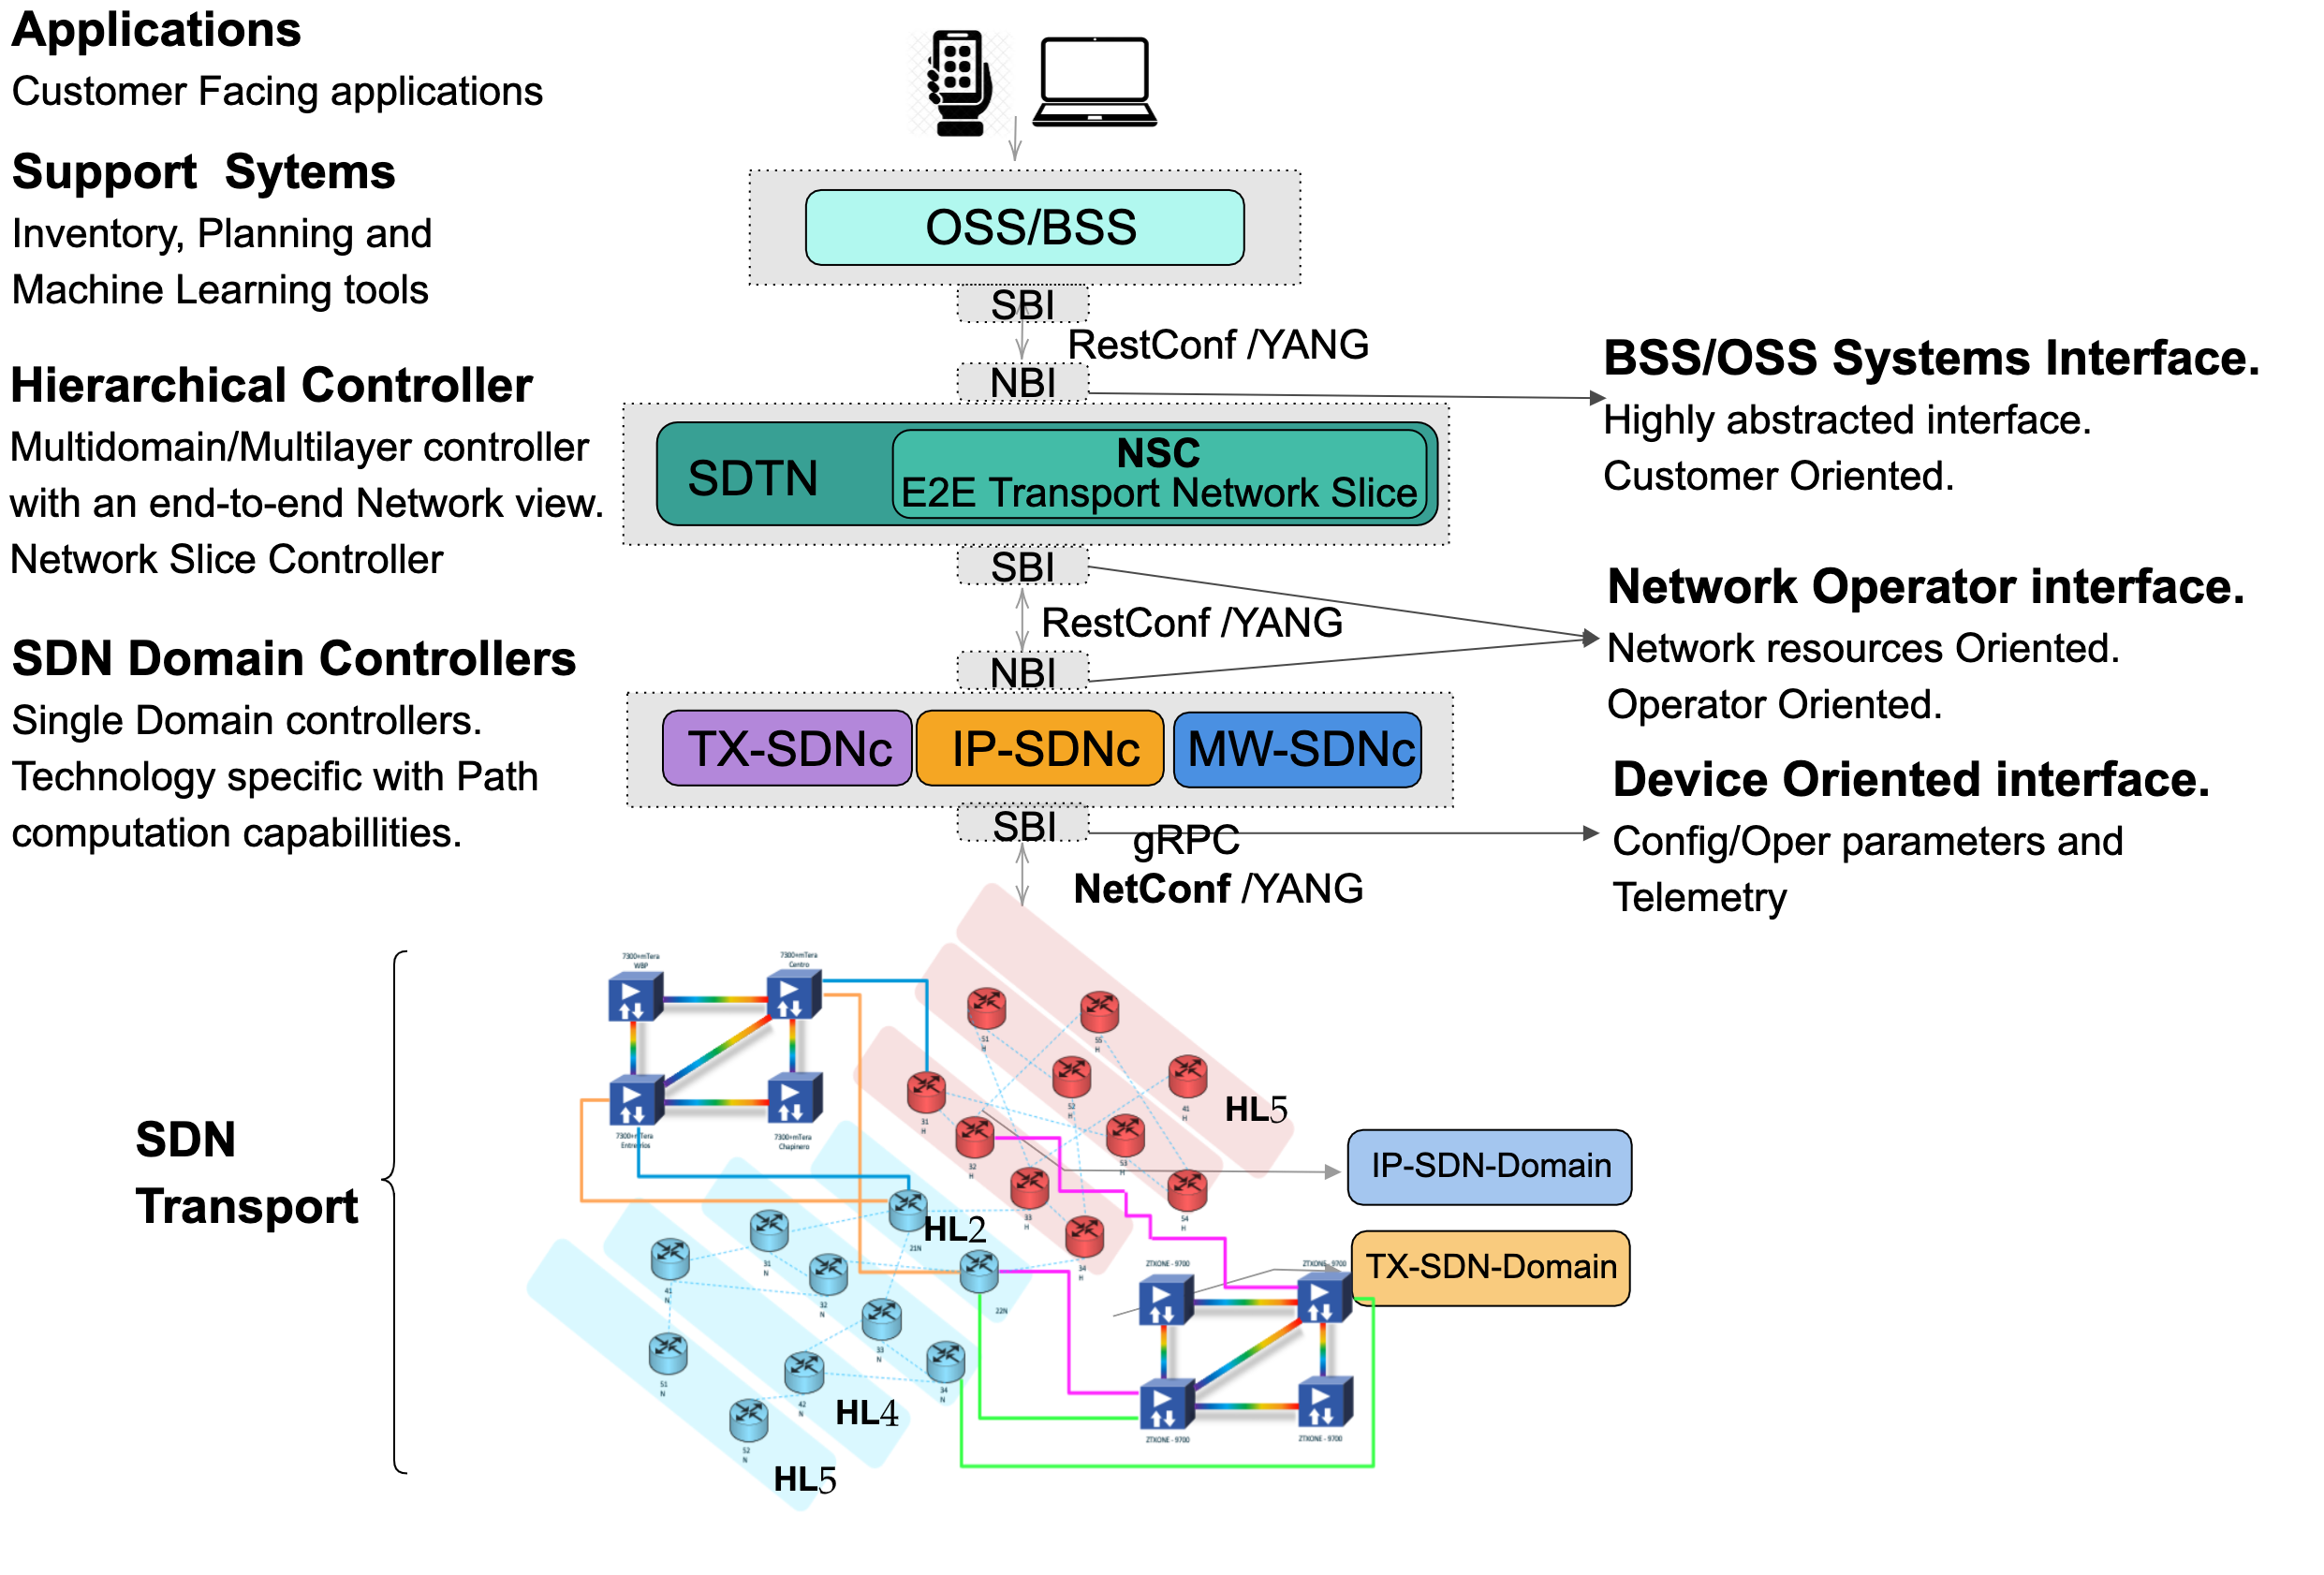
\includegraphics[width=\linewidth]{Figs/diagram-1.png}
\caption{Overall proposed architecture}
\label{fig:architecture}
\end{figure}

\Cref{fig:architecture} shows the network scheme of the i\uppercase{FUSION} architecture in terms of components and relationships among them. The following sections define each of the structural pillars in the architecture, including its role in network slicing.

%\begin{figure}[tb]%[htdp]
%\centering
%	\centering
%		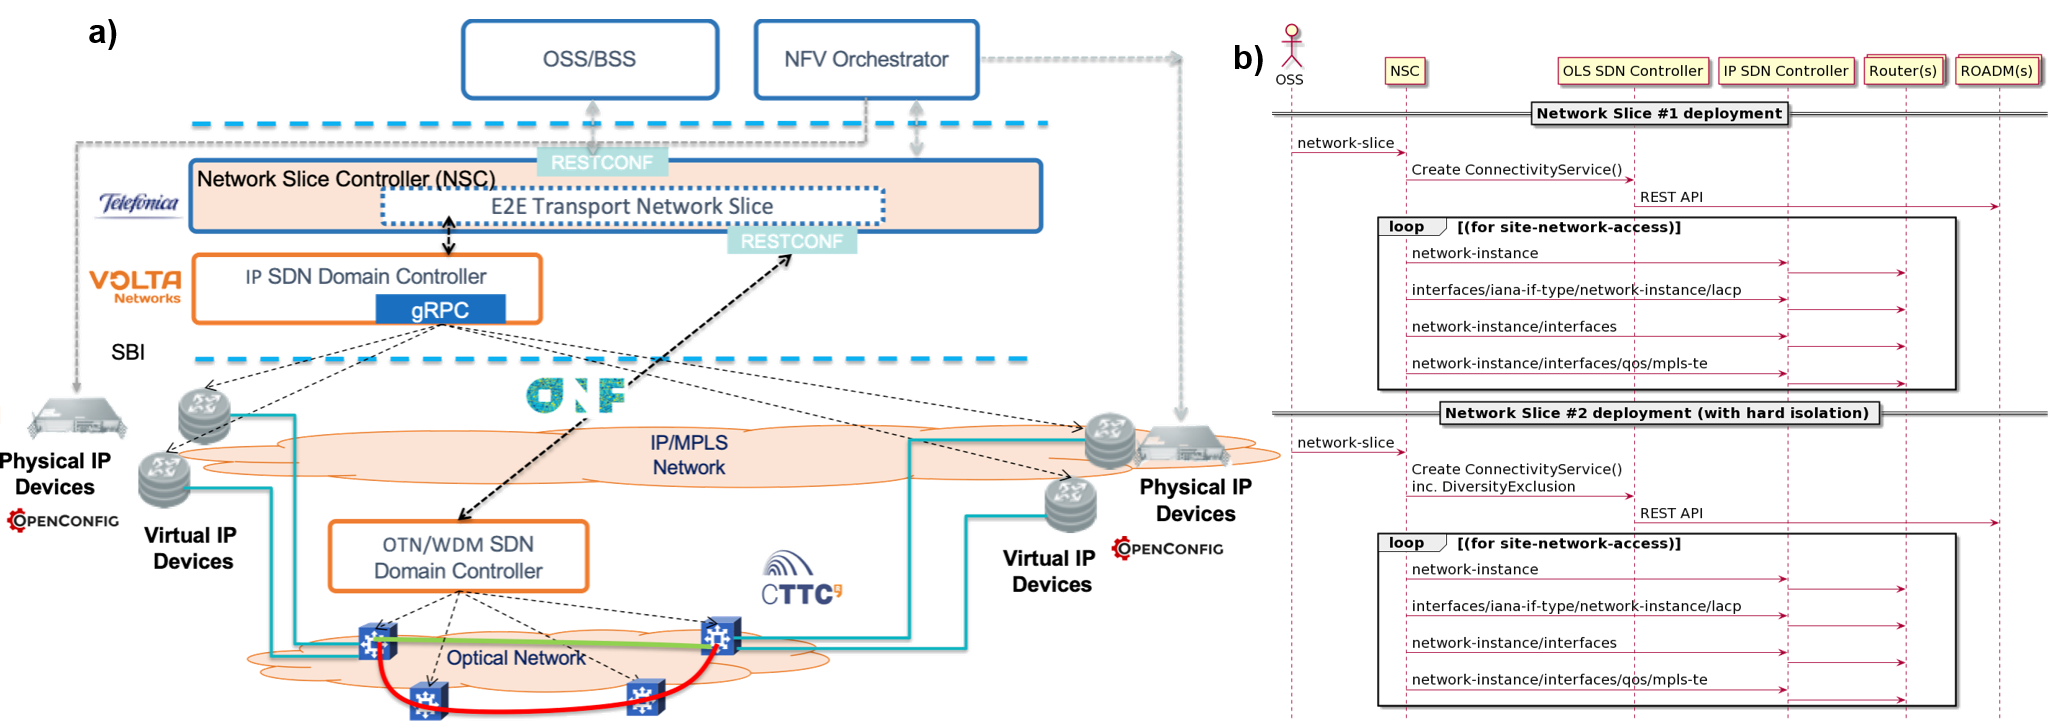
\includegraphics[width=\linewidth]{Figs/arch.png}
%\caption{a) Overall proposed architecture; and b) Sequence diagram for multiple network slice deployment with isolation characteristics.}
%\label{fig:scheme}
%\end{figure}

%Figure \ref{fig:scheme}.b shows the proposed workflow to deploy hard and soft transport network slices. In the workflow, two isolated network slices are deployed. The first one allocates a connectivity service to interconnect both IP layer domains (see for reference Figure \ref{fig:scheme}.a). This triggers the necessary optical configuration mechanism to each of the underlying ROADMs (e.g., using OpenROADM protocol). 

%Once the connectivity service has been established, the NSC is responsible for requesting to IP SDN domain controller the necessary virtual routers (in the proposed scenario, two site-network-access are configured, one network instance on each site). Link Aggregation Control Protocol (LACP) is configured to each network instance. Then interfaces are aggregated and properly configured using dedicated VLAN or MPLS-TE mechanisms. 

%When a new isolated slice is requested, NSC can request a dedicated and isolated connectivity service to the underlying optical SDN controller. Figure \ref{fig:results}.b details the available connectivity constraint to provide disjoint path selection using ONF Transport API. It consists of including a diversity exclusion constraint with the previous connectivity service identifier. Later, at IP layer novel virtual routers are deployed to provide the requested degree of isolation.


\subsection{Software Defined Transport Network Controller} 
\label{sec:ifusionarch}

The Software-Defined Transport Network Controller is a functional block with the following purposes \cite{contreras2019ifusion}; It is The main entry point from the OSS/BSS systems to the network. It is in charge of coordinating/providing services through several domains and layers. It has the multi-layer/multi-domain topological view of the network. The SDTN controller can split requirements based on the technological requirements. During this process, the SDTN controller can add/assign logical resources to be used by the network at the service implementation. The SDTN controller have two RESTCONF interfaces, one to process the OSS/BSS systems' requirements and one to send the specific requests to the domain controllers. TeraFlow project \cite{vilalta21eucnc} is proposing the development of a cloud-native SDN controller that will serve as SDTN.


The SDTN controller can have incorporated the Network Slice Controller as a working piece of its implementation.

\subsection{Network Slice Controller} 

The Network Slice Controller (NSC) effectuates a transport network slice in the underlying transport infrastructure, manages and control the state of resources and topologies associated with it. The NSC receives a transport network slice request from the Operation Support System and Business Support System (OSS/BSS). The NSC runs an internal workflow for transport network slice life-cycle management and interacts with underlying IP and Optical Domain controllers via a RESTCONF client. As described in the following sections, depending on the NSC location in the architecture, the NSC will delegate to SDN Domain controllers to configure the network (\cref{sec:instantiation}.a and \cref{sec:instantiation}.b) or make it directly through a NETCONF SBI (\cref{sec:instantiation}.c). 

The network slice controller is the key building block for control and management of network slice. It provides the creation/modification/deletion, monitoring an optimization of network slices in a multi-domain, a multi-technology and multi-vendor environment. It has two main functionalities defined in \cite{contreras2020slice,slicing2021framework}:
\begin{itemize}
    \item \textit{Map}: The NSC must Map the Network Slice requests to the underlying technology-specific infrastructure. Accordingly, It maintains a record of the mapping from user requests to slice instantiations, as needed to allow for subsequent control functions like modification or deletion.
    \item  \textit{Realize}: The NSC should realize the network slice request using its SBI interface against the domain controllers in either physical or logical connectivity through VPNs or various tunnelling technologies such as Segment Routing, MPLS, etc. 
\end{itemize}

\subsection{Network Domain Controller} 

The network domain controller (SDN Controller) is in charge of network elements (network domain). It has standard southbound interfaces to communicate with the network elements. The Domain controller SBI relies on using the Network configuration protocol (NETCONF) to interact with the underlying technology's network elements. The SDN controller also has a northbound interface to communicate with the SDTN controller or the OSS/BSS Systems using RESTCONF.

\subsection{Yang Models for Network Controllers}

As described until now, the three control elements: SDTN controller, Network Slicing Controller and Network Domain controllers, has standard SBI and NBI interfaces to communicate between them and against the network or the OSS/BSS systems. The standard interfaces are composed of selecting a protocol to transfer the data and YANG data models to define how the message is formed. For that sense, the YANG modelling activities have acquired significant relevance across the standardization entities. To such an extent that by 2019, the Number of correctly extracted YANG models from IETF drafts was 283, in the Broadband forum was 214, and in Openconfig was 137 \cite{benoit2020yang}; similarly, other organizations like the MEF, 3GPP or ONF produced YANG data models to describe technologies, protocols or connectivity services as well. Thus, navigating through the massive set of YANGs available and selecting the suitable pack of data models to define each functional block's interfaces becomes an essential task from the architectural definitions point of view. 

To request and after instantiate the network slices a set of these data models are described as the experimental base of this work are described in the \cref{TAB2:models}.

\begin{table}[htb]
\caption{Set of these data models are described as the experimental base of this work}
\begin{tabular}{|l|l|l|}
\hline
\textbf{Models}  & 
\textbf{Description}  & 
\textbf{Example} \\ \hline \hline 
LxVPN  & 
\begin{tabular}[c]{@{}l@{}}These models describe a VPN service \\ from the customer or network \\ operator point of view.\\\end{tabular} &
\begin{tabular}[c]{@{}l@{}}L3SM: \cite{l3sm2017Litkowski} \\ L2SM: \cite{wen2018yang}\\ L3NM:\cite{Aguado.2021l3nm} \\ L2SM: \cite{barguil2021l2nm}\end{tabular} \\ \hline

Traffic Engineering & 
\begin{tabular}[c]{@{}l@{}}These models allow to manipulate \\ Traffic Engineering tunnels \\ within the network segment. \\ Technology-specific extensions \\ allow to work with a desired technology \\ (e.g. MPLS RSVP-TE tunnels, \\ Segment Routing paths,\\OTN tunnels, etc.)\\\end{tabular} & 
\begin{tabular}[c]{@{}l@{}}TE:\cite{te2021Saad}\\ TE Topology:\cite{ietf2021tetopology,ietf2021tel3topology}\end{tabular} \\ \hline

\begin{tabular}[c]{@{}l@{}}TE Service Mapping \\ extensions\end{tabular} & \begin{tabular}[c]{@{}l@{}}These extensions allow to specify \\ for LxVPN the details of an underlay \\ based on Traffic Engineering\\\end{tabular}& 
\begin{tabular}[c]{@{}l@{}}Service \\Mapping: \cite{teas2021servicemapping} \end{tabular} \\\hline

\begin{tabular}[c]{@{}l@{}}ACLs and \\ Routing policies\end{tabular}    & \begin{tabular}[c]{@{}l@{}}Even though ACLs and routing policies\\ are device models,\\It's exposure in the NBI of a domain\\controller allows to provide\\an additional granularity\\that the network domain\\controller is not able to infer on its own.\end{tabular}                 & \begin{tabular}[c]{@{}l@{}}ACL: \cite{ietf2019acl}\\ Routing\\ Policy:\cite{ietf2021routingpolicy,ietf2021bgppolicy}\end{tabular}\\ \hline

OTN  & \begin{tabular}[c]{@{}l@{}}As a part of the transport network,\\
   OTN can provide hard pipes \\with guaranteed data isolation and\\
   deterministic low latency, \\which are highly demanded in the Service\\
   Level Agreement (SLA).\\\end{tabular} & \begin{tabular}[c]{@{}l@{}}OTN Slice: \cite{ietf2021otnslicing}\end{tabular}\\ \hline

Slicing  & \begin{tabular}[c]{@{}l@{}}Set of data models available to map \\ and realize the network Slices.\\ \end{tabular} & \begin{tabular}[c]{@{}l@{}}Network Slice\\ NBI:\cite{slicing2021framework,contreras2020slice}\\ \end{tabular} \\ \hline
\end{tabular}
\label{TAB2:models}
\end{table}

%%%%%%%%%%%%%%%%%%%%%%%%%%%%%%%%%%%%%%%%%%
\subsection{Instantiating of Network Slices in SDN transport networks}
\label{sec:instantiation}

As described before in the \cref{sec:ifusionarch}, the OSS/BSS systems may request the deployment of a new network slices with certain transport characteristics. Each network slice must be isolated from any other network slices or different services delivered to particular customers and naturally, other network slices or services must not negatively impact the requested transport network slice's delivery. 

To provide this isolation and instantiate the slice in the network there are certain implementation options ranging from softer to hardest grades of isolation, as follow:  

\begin{itemize}
    \item No-isolation: meaning that slices are not separated.
    \item Logical-isolation: where slices are logically separated, only a certain degree of isolation is performed through QoS mechanisms.
    \item Service-isolation: where virtual resources and NFs are shared.
    \item Process-isolation: where slices include process and threads isolation. 
    \item Virtual-resource-isolation: where slices have dedicated virtual resources.
     \item Network-functions-isolation: where Network Function (NF) are dedicated to a single network slice.   
    \item Physical-isolation: where slices are completely physically separated, for example, in different locations.
    \item Physical-network-isolation: where slices contain physically separated links. 
\end{itemize}

As the isolation grade is a significant constraint to consider for the network slice implementation, the selected network infrastructure and the control elements selected would generate different sets of capabilities in the Network Slice Controller. \Cref{fig:instantiation} describes three of the possibilities analyzed from the point of view of the mapping and realization tasks of the Network Slice Controller:

\begin{enumerate}[label=(\alph*)]

\item \textbf{Network Slice Controller as part of the hierarchical controller:}
When the Network Slice Controller is a Hierarchical SDN controller module, the NSC's and the Hierarchical Network Controller should share the same internal data and the same NBI. Thus, to process the customer, view the H-SDN module must be able to:

\begin{itemize}
    \item \textit{Map}: The customer request received using the must be processed by the NCS. The mapping process takes the network-slice SLAs selected by the customer to available Routing Policies and Forwarding policies.
    
    \item  \textit{Realize}: Create necessary network requests. The slice's realization can be translated into one or several LXNM Network requests, depending on the number of underlay controllers. Thus, the NCS must have a complete view of the network to map the orders and distribute them across domains. The realization should include the expansion/selection of Forwarding Policies, Routing Policies, VPN policies, and Underlay transport preference.    
\end{itemize}

To maintain the data coherence between the control layers, the \texttt{network-slice-id} used  must be directly mapped to the  \texttt{transport-instance-id} at the VPN-Node level.     
    \item \textbf{Network Slice Controller as an stand-alone controller:}

When the Network Slice Controller is a stand-alone controller module, the NSC's should perform the same two tasks described before:

\begin{itemize}
    \item \textit{Map}: Process the customer request. The customer request can be sent using the [draft-liu-teas-transport-network-slice-yang-01]. This draft allows the topology mapping of the Slice request. 
    
    \item  \textit{Realize}: Create necessary network requests. The slice's realization will be translated into one LXNM Network request. As the NCS has a topological view of the network, the realization can include the customer's traffic engineering transport preferences and policies.
\end{itemize}

    \item \textbf{Network Slice Controller at the domain controller level:}

The Network Slice Controller can at the same level as the network domain controllers. The SDTN controller should handle the slices request, and the realization can be done by the NSC directly communicating with the Network Elements. The SDTN controller should create unified network views, including each transport domain and the network slices.

\begin{itemize}

    \item \textit{Map}: The SDTN would Process the customer request. The customer request can be sent using the [draft-liu-teas-transport-network-slice-yang-01]. This draft allows the topology mapping of the Slice request. 
    
    \item \textit{Realize}: The realization can be done by the NCS controller applying the service logic to create policies directly on the Network elements. The SDTN should handle the shared resources management between domains. 
\end{itemize}    
    
    \item \textbf{Network Slice Controller as part of the domain controller:}
    
When the Network Slice Controller is part of the domain controller, the OSS/BSS systems process the Slices requests and introduce the network abstraction layer. At the network level, the same device data model would be used in the NBI and SBI of the SDN controller. The direct translation would reduce the service logic implemented at the SDN controller level, grouping the mapping and translation into a single task. :

\begin{itemize}
    \item  \textit{Map & Realize}:The mapping and realization can be done by the Domain controller applying the service logic to create policies directly on the Network elements.
\end{itemize}

\end{enumerate}

\begin{figure}[htb]%[htdp]
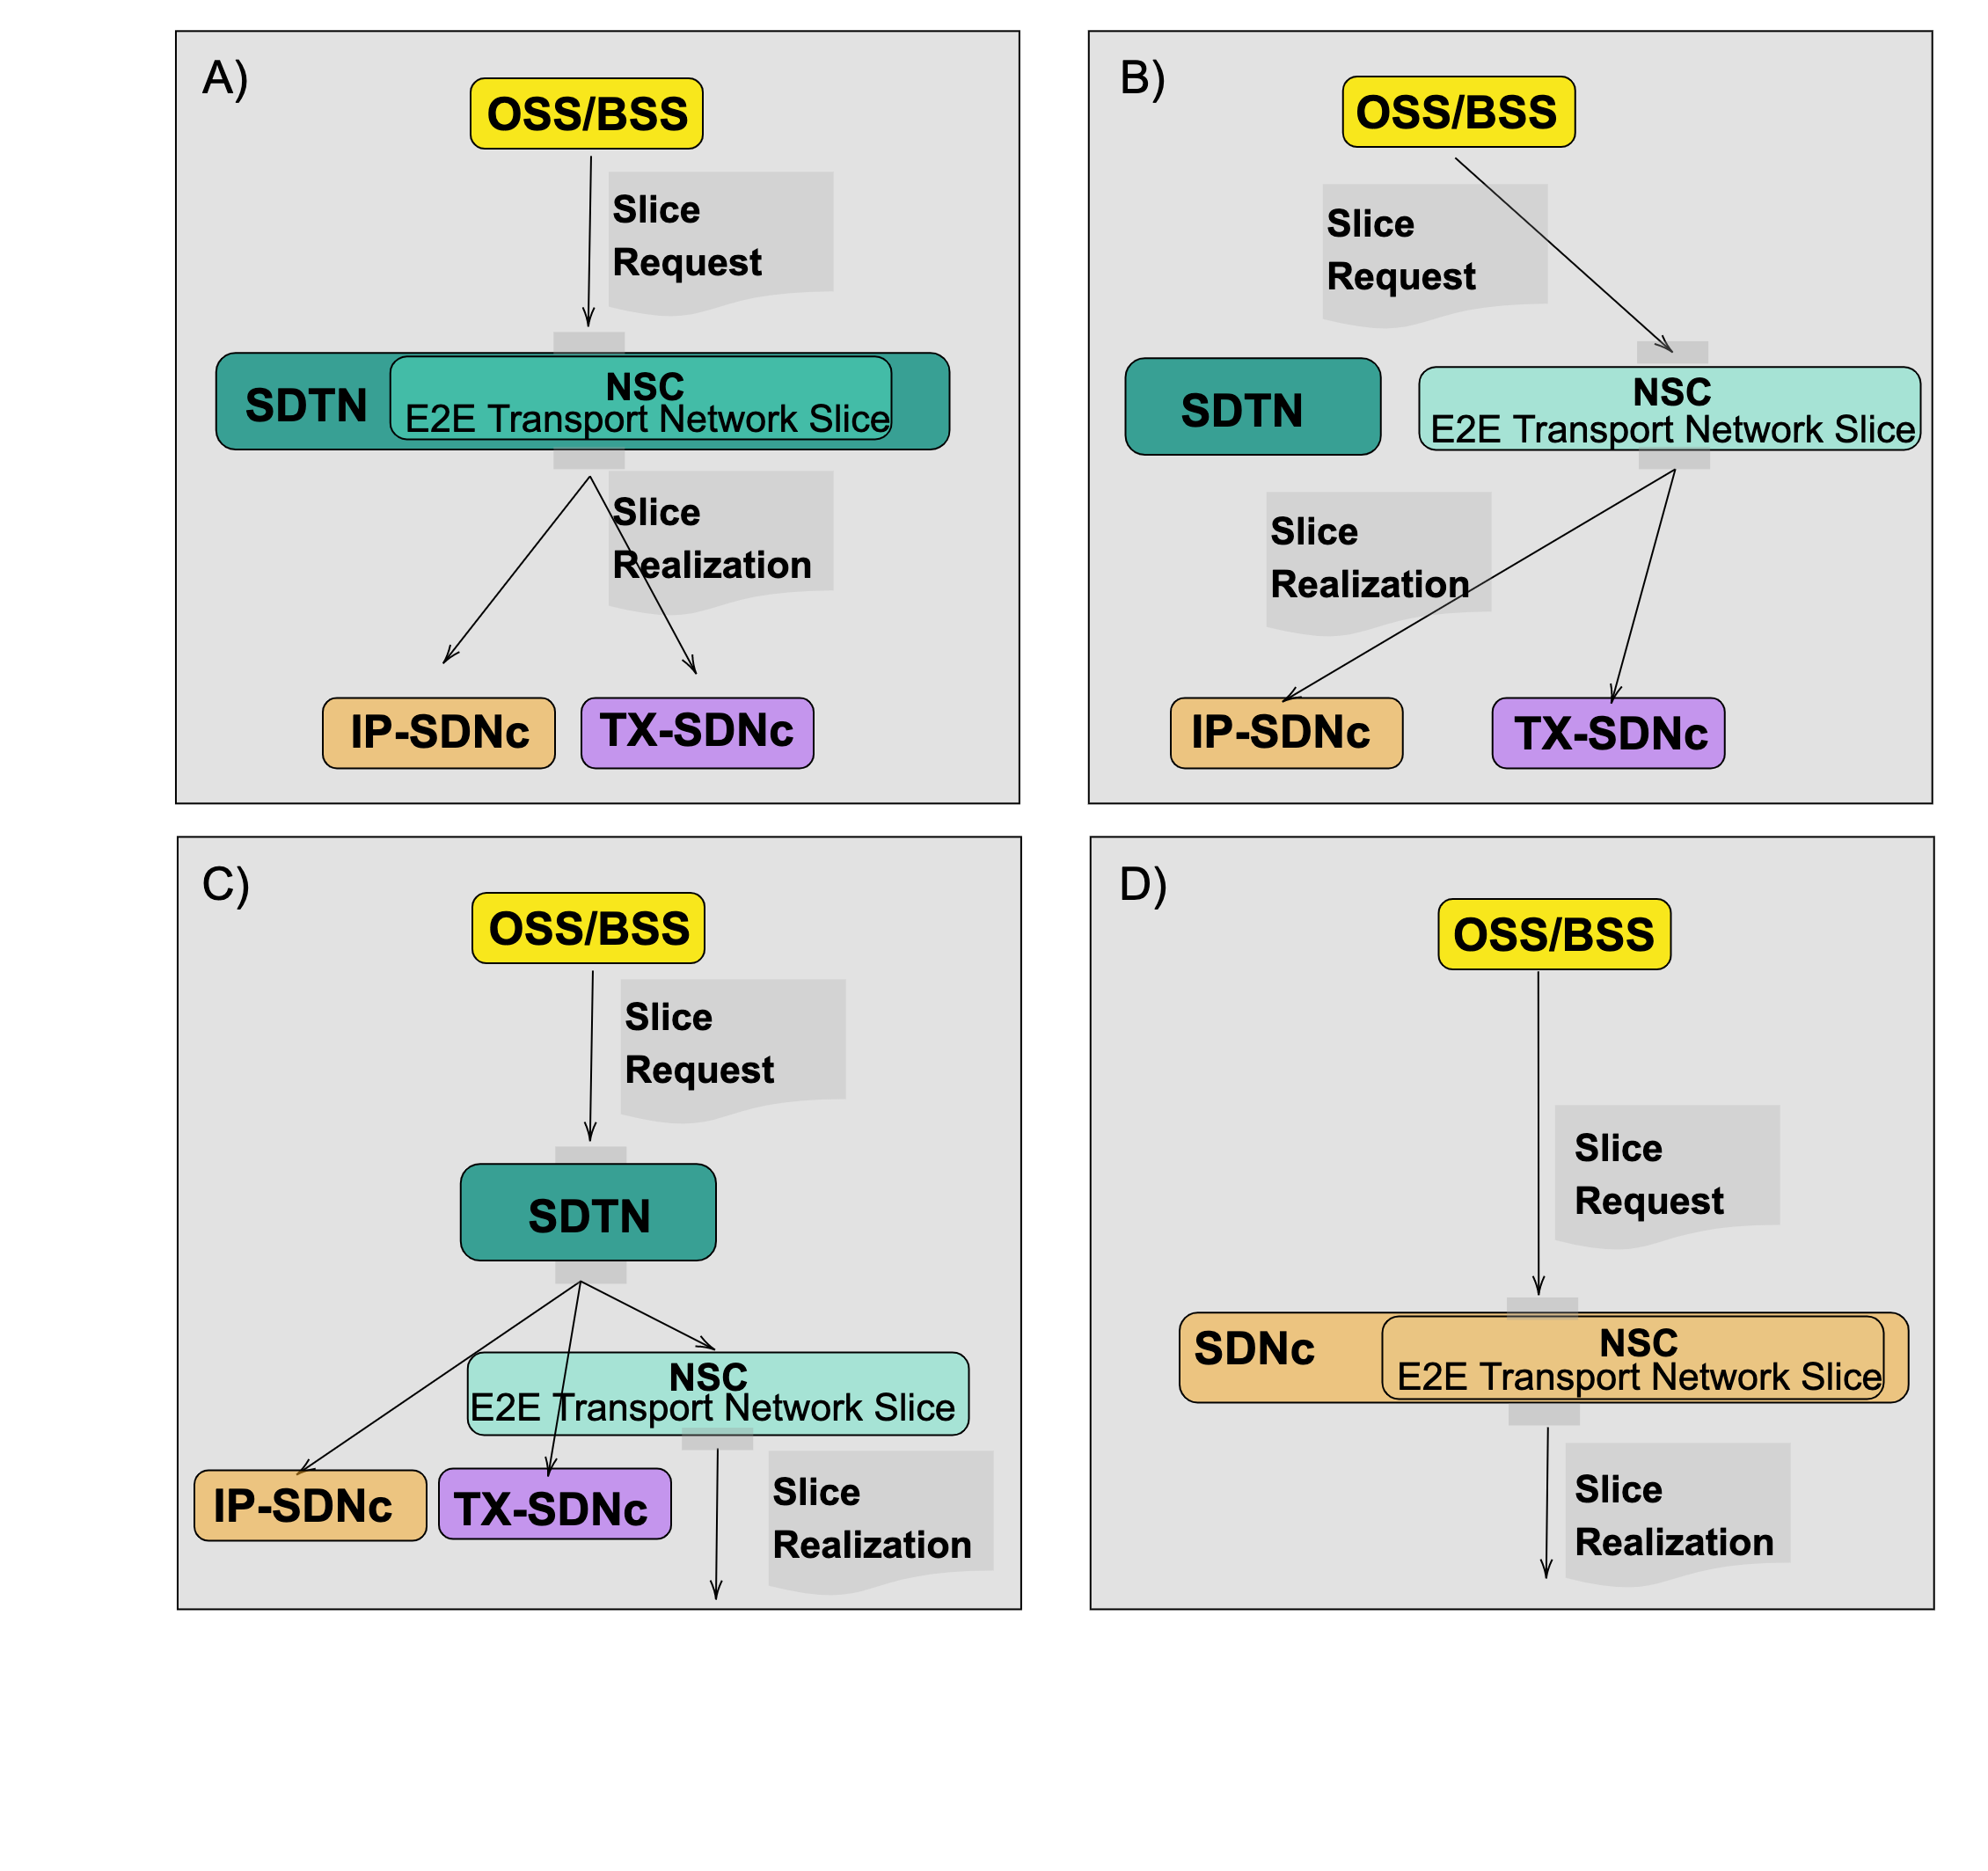
\includegraphics[width=\linewidth]{Figs/diagram-2.png}
\caption{Possible Network Slice instantation in a service provider network.A) Network Slice Controller as part of the hierarchical controller, B) Network Slice Controller as an independent hierarchical controller, C) Network Slice Controller as an independent domain controller and D) Network Slice Controller as part of the domain controller}
\label{fig:instantiation}
\end{figure}

%%%%%%%%%%%%%%%%%%%%%%%%%%%%%%%%%%%%%%%%%%
\section{Experimental Validation}
\label{sec:results}

The experimental testbed has been distributed between Telefónica and CTTC laboratory premises, as depicted in Figure \ref{fig:scheme}. The testbed includes two layers, a control layer and a transport layer.  

Telefonica and CTTC deployed a control layer composed of three relevant items. First, to receive all the service requests, a Network Slice Controller was developed as part of the SDTN controller. Second, to interact with the transport domains, the testbed included Two (2) controllers, one for IP and one for Optical. To configure the routers, the IP SDN Controller used gRPC, while the Optical SDN controller used Netconf with T-API for the configuration tasks.

The physical transport layer was composed of:

\begin{itemize}
    \item Two (2) 7316 Edgecore switches running ONIE.
    \item Two (2) Spirent traffic generator.
    \item Four (4) Flexi-grid DWDM nodes.
\end{itemize}

The  Edgecore used a 10 Gigabit Ethernet (10G) interface for the connection against the Spirent testers and 1G interfaces to the Optical devices. Furthermore, on each Edgecore, two (2) separate virtual routers were configured to test redundancy and route filtering between the ends. The Network Operating system (NOS) running on the virtual-routers were volta-stack deployment version \texttt{20.4-2-36-g0ba8807}. 

\begin{figure}[tb]%[htdp]
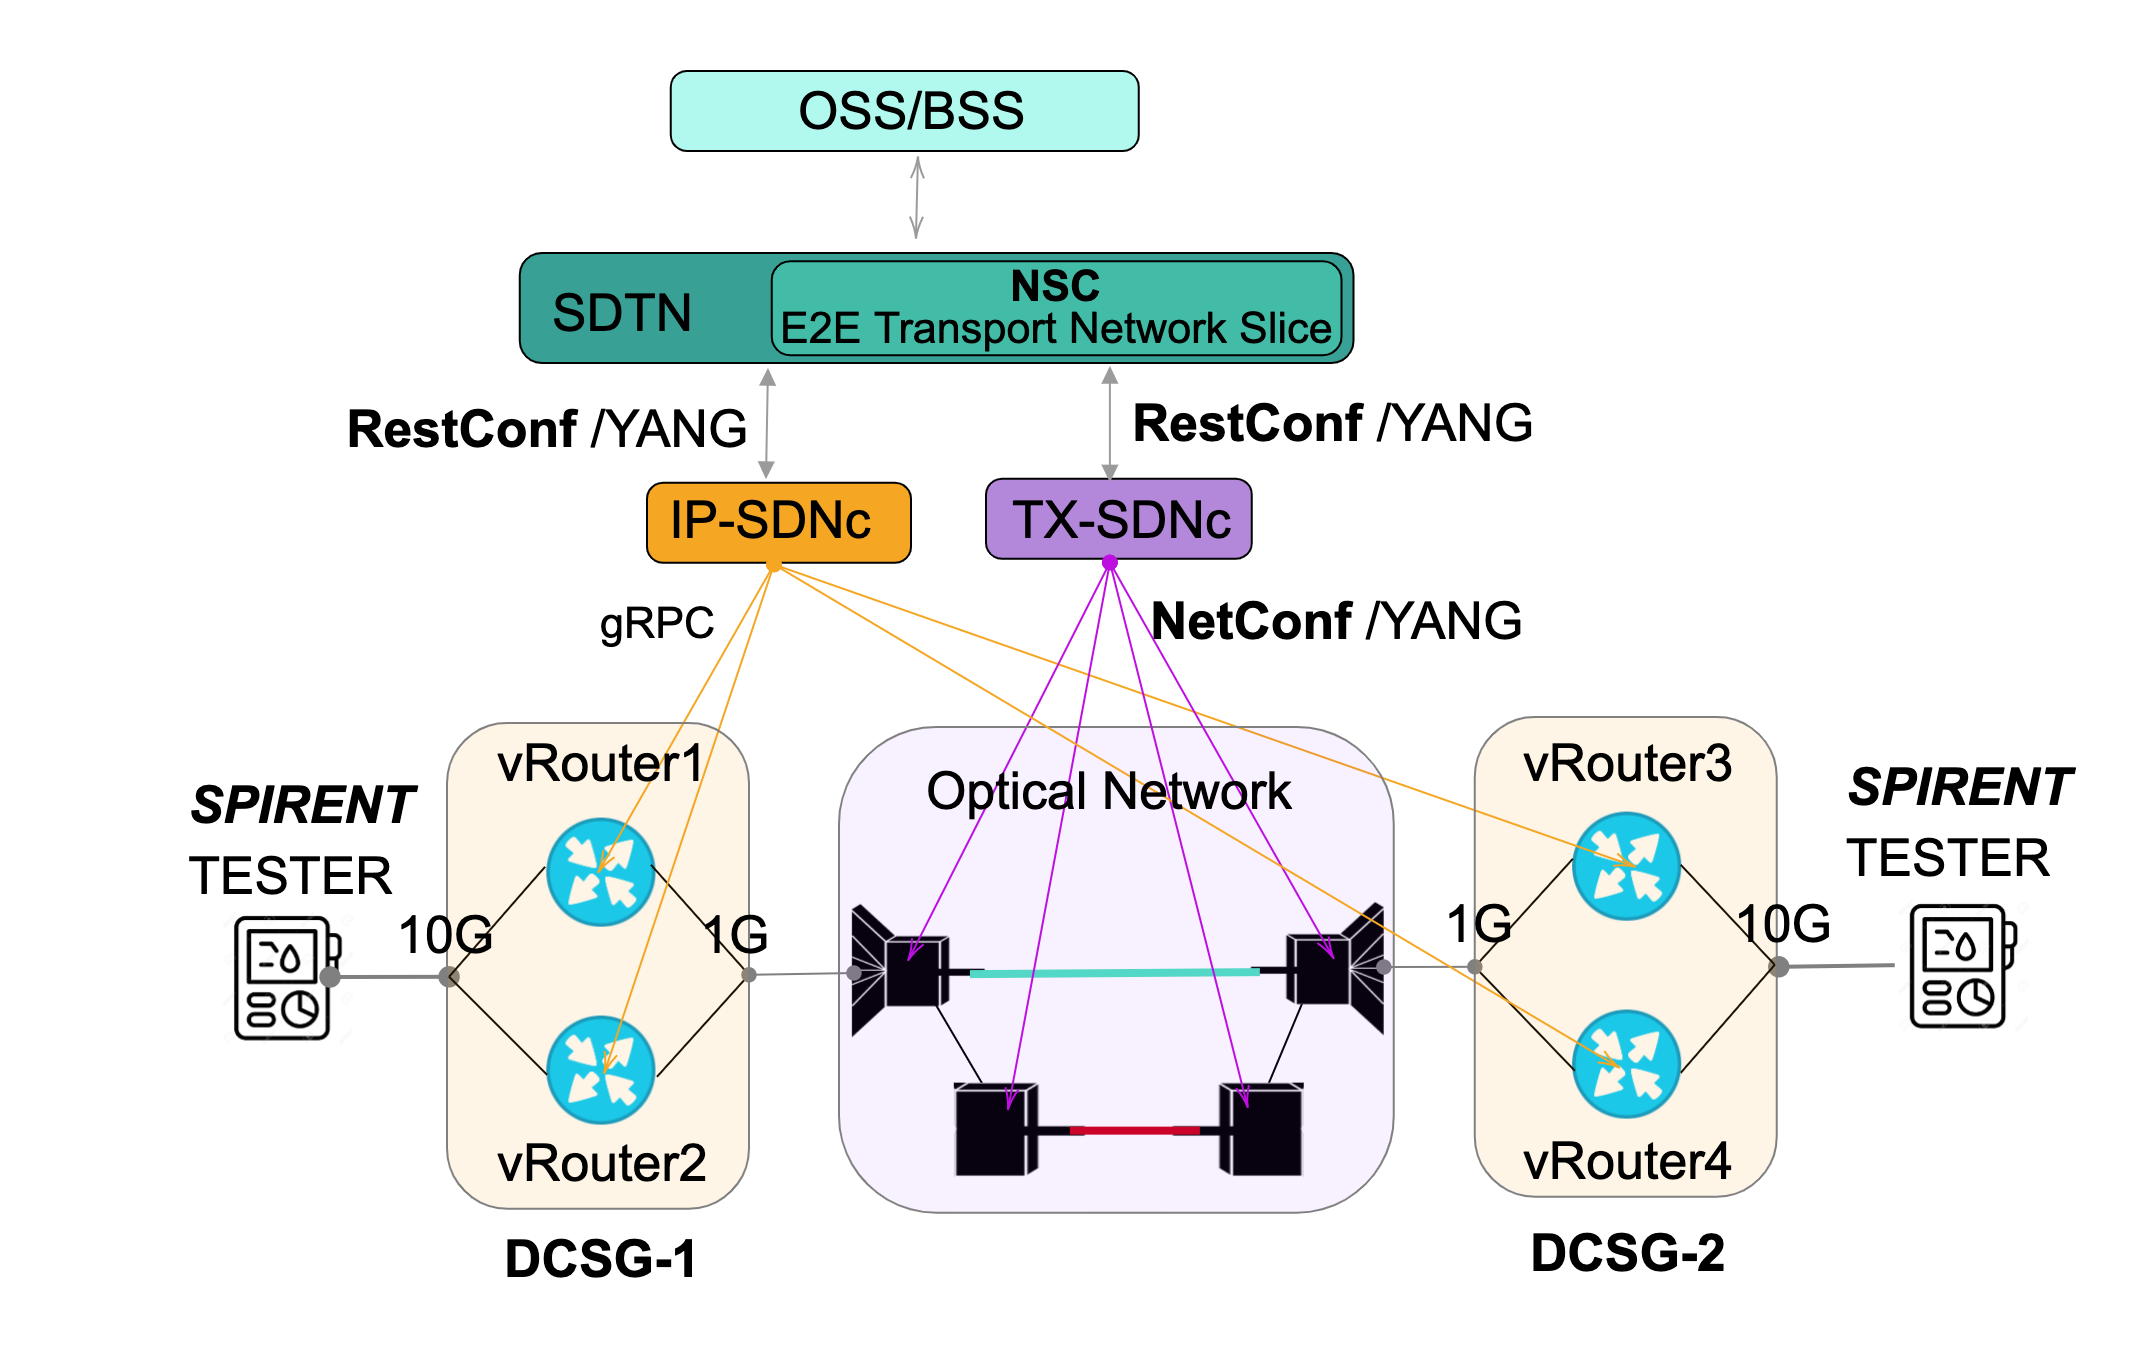
\includegraphics[width=\linewidth]{Figs/diagram-6.png}
\caption{Network Design, including the Logical and Physical Infrastructure to support the test cases.}
\label{fig:scheme}
\end{figure}

As we have described previously, there are several requirements for network automation for network slicing. However, a service provider can not all treat all the needs in the same way. Thus, a set of use cases were designed and executed as part of the whole testing process, the use cases were the following:

\begin{enumerate}
    \item Slice Creation: To request a Standards-Based and Model-Driven isolated Network Slices using . The SDTN controller would receive and translate the network slice service into specific per domain requests as follows:
    \begin{enumerate}
        \item  L3VPN service creation: In this use case, each network slice request requires an L3VPN service creation; thus, each L3VPN service would map to a single network slice. The endpoints defined in the slice request would map to Virtual Router and Forwarding (VRFs) instances on the virtual routers. The Yang data model used for the SDTN requests the L3VPN services to the IP domain controller was the L3NM \cite{Aguado.2021l3nm}.
        \item  DWDM connectivity: The T-API \cite{vilalta2018experimental} was used to create a new connectivity service in the transport network to enable the L2-L1 communication between the network slice endpoints. 
    \end{enumerate}
    \item Add Prefixes and destroy: The second use case expects to validate the IP connectivity between the network slices. Hence the Spirent testers announced a set of 5k IP prefixes through the prior created network slices. Afterwards, the testers make an automatic IP reachability test and a CLI route redistribution validation. Once the route propagation was validated, the testing team stopped all the Spirent prefixes' announcement, and a new automatic connectivity test was done.  
        \begin{enumerate}
            \item Device recovery test:  The third use case was to verify the network slices service continuity so. The testing team manually rebooted all the DCSGs. Once the devices got online again, we have checked the service status with a measurement of the service restoration time.
      \end{enumerate}
\end{enumerate}

\subsection{Slice Creation}

The iFusion architecture enhancement proposed for this paper performs the management of services and resources through the use of information models that capture the definitions of managed entities in terms of attributes and supported operations. Hence, a set of Yang Data models has been defined to render and realize a network slice between each of the control entities. The workflow proposed used postman to simulate, the network slice creation requests. The YANG data-model used for this request was defined in \cite{liu2020slice}. It includes the endpoints, the customer information and the service level agreement of the slice requests. The PE-CE and the end-to-end connectivity protocols for the network slice realization was automatically expanded by the SDTN controller and received by the IP SDN controller to properly configure the network elements.  Each network slice, The workflow can be seen in the \cref{fig:slicecreation}.

\begin{figure}[htb]
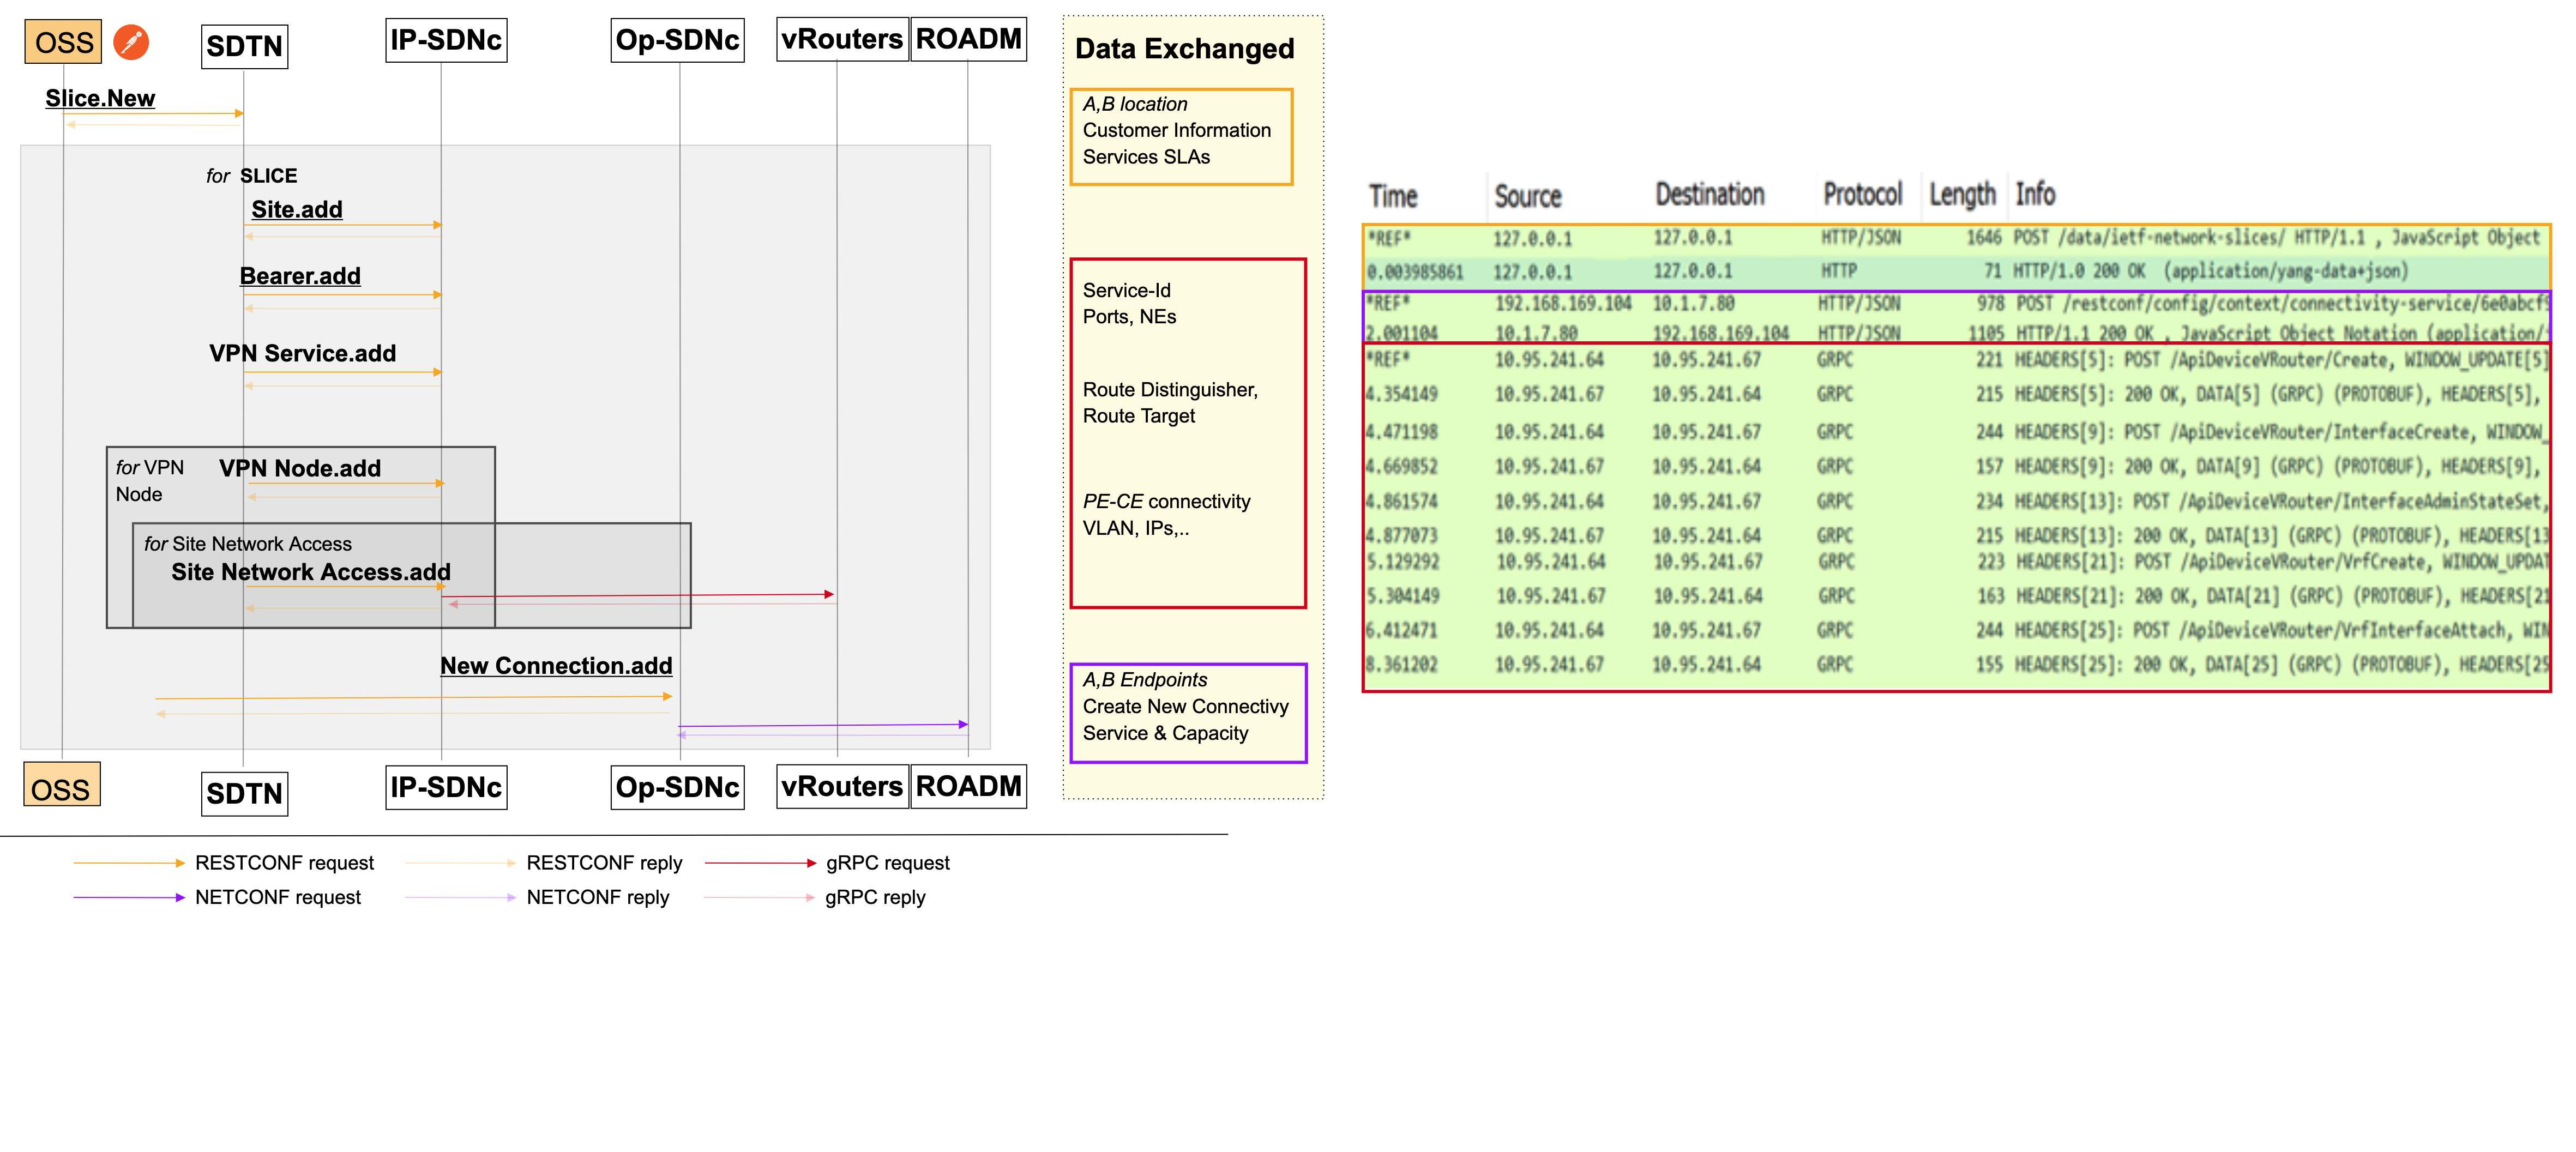
\includegraphics[width=\linewidth]{Figs/slicecreation.png}
\caption{Workflow used to instantiate the network slices in the network. From Postman, a user sends a slice request to the SDTN controller. The SDTN controller automatically split the request based on technological requirements. The L3NM and the T-API are used for the IP and Optical domains, respectively.}
\label{fig:slicecreation}
\end{figure}


\subsection{Add Prefixes and destroy}

Once the domain controller realized the network slices, and we have validated the service status. The next step vas to verify the correct establishment of the data-plane sessions. Thus, the Spirent testers added 5k prefixes to each of the services(VRF-Blue and VRF-Red). To confirm the status of each service, we have captured the virtual routers BGP information, as depicted in \cref{fig:sliceresults}, where each VRF has 5002 prefixes received (PfxRcd). 

\begin{figure}[htb]
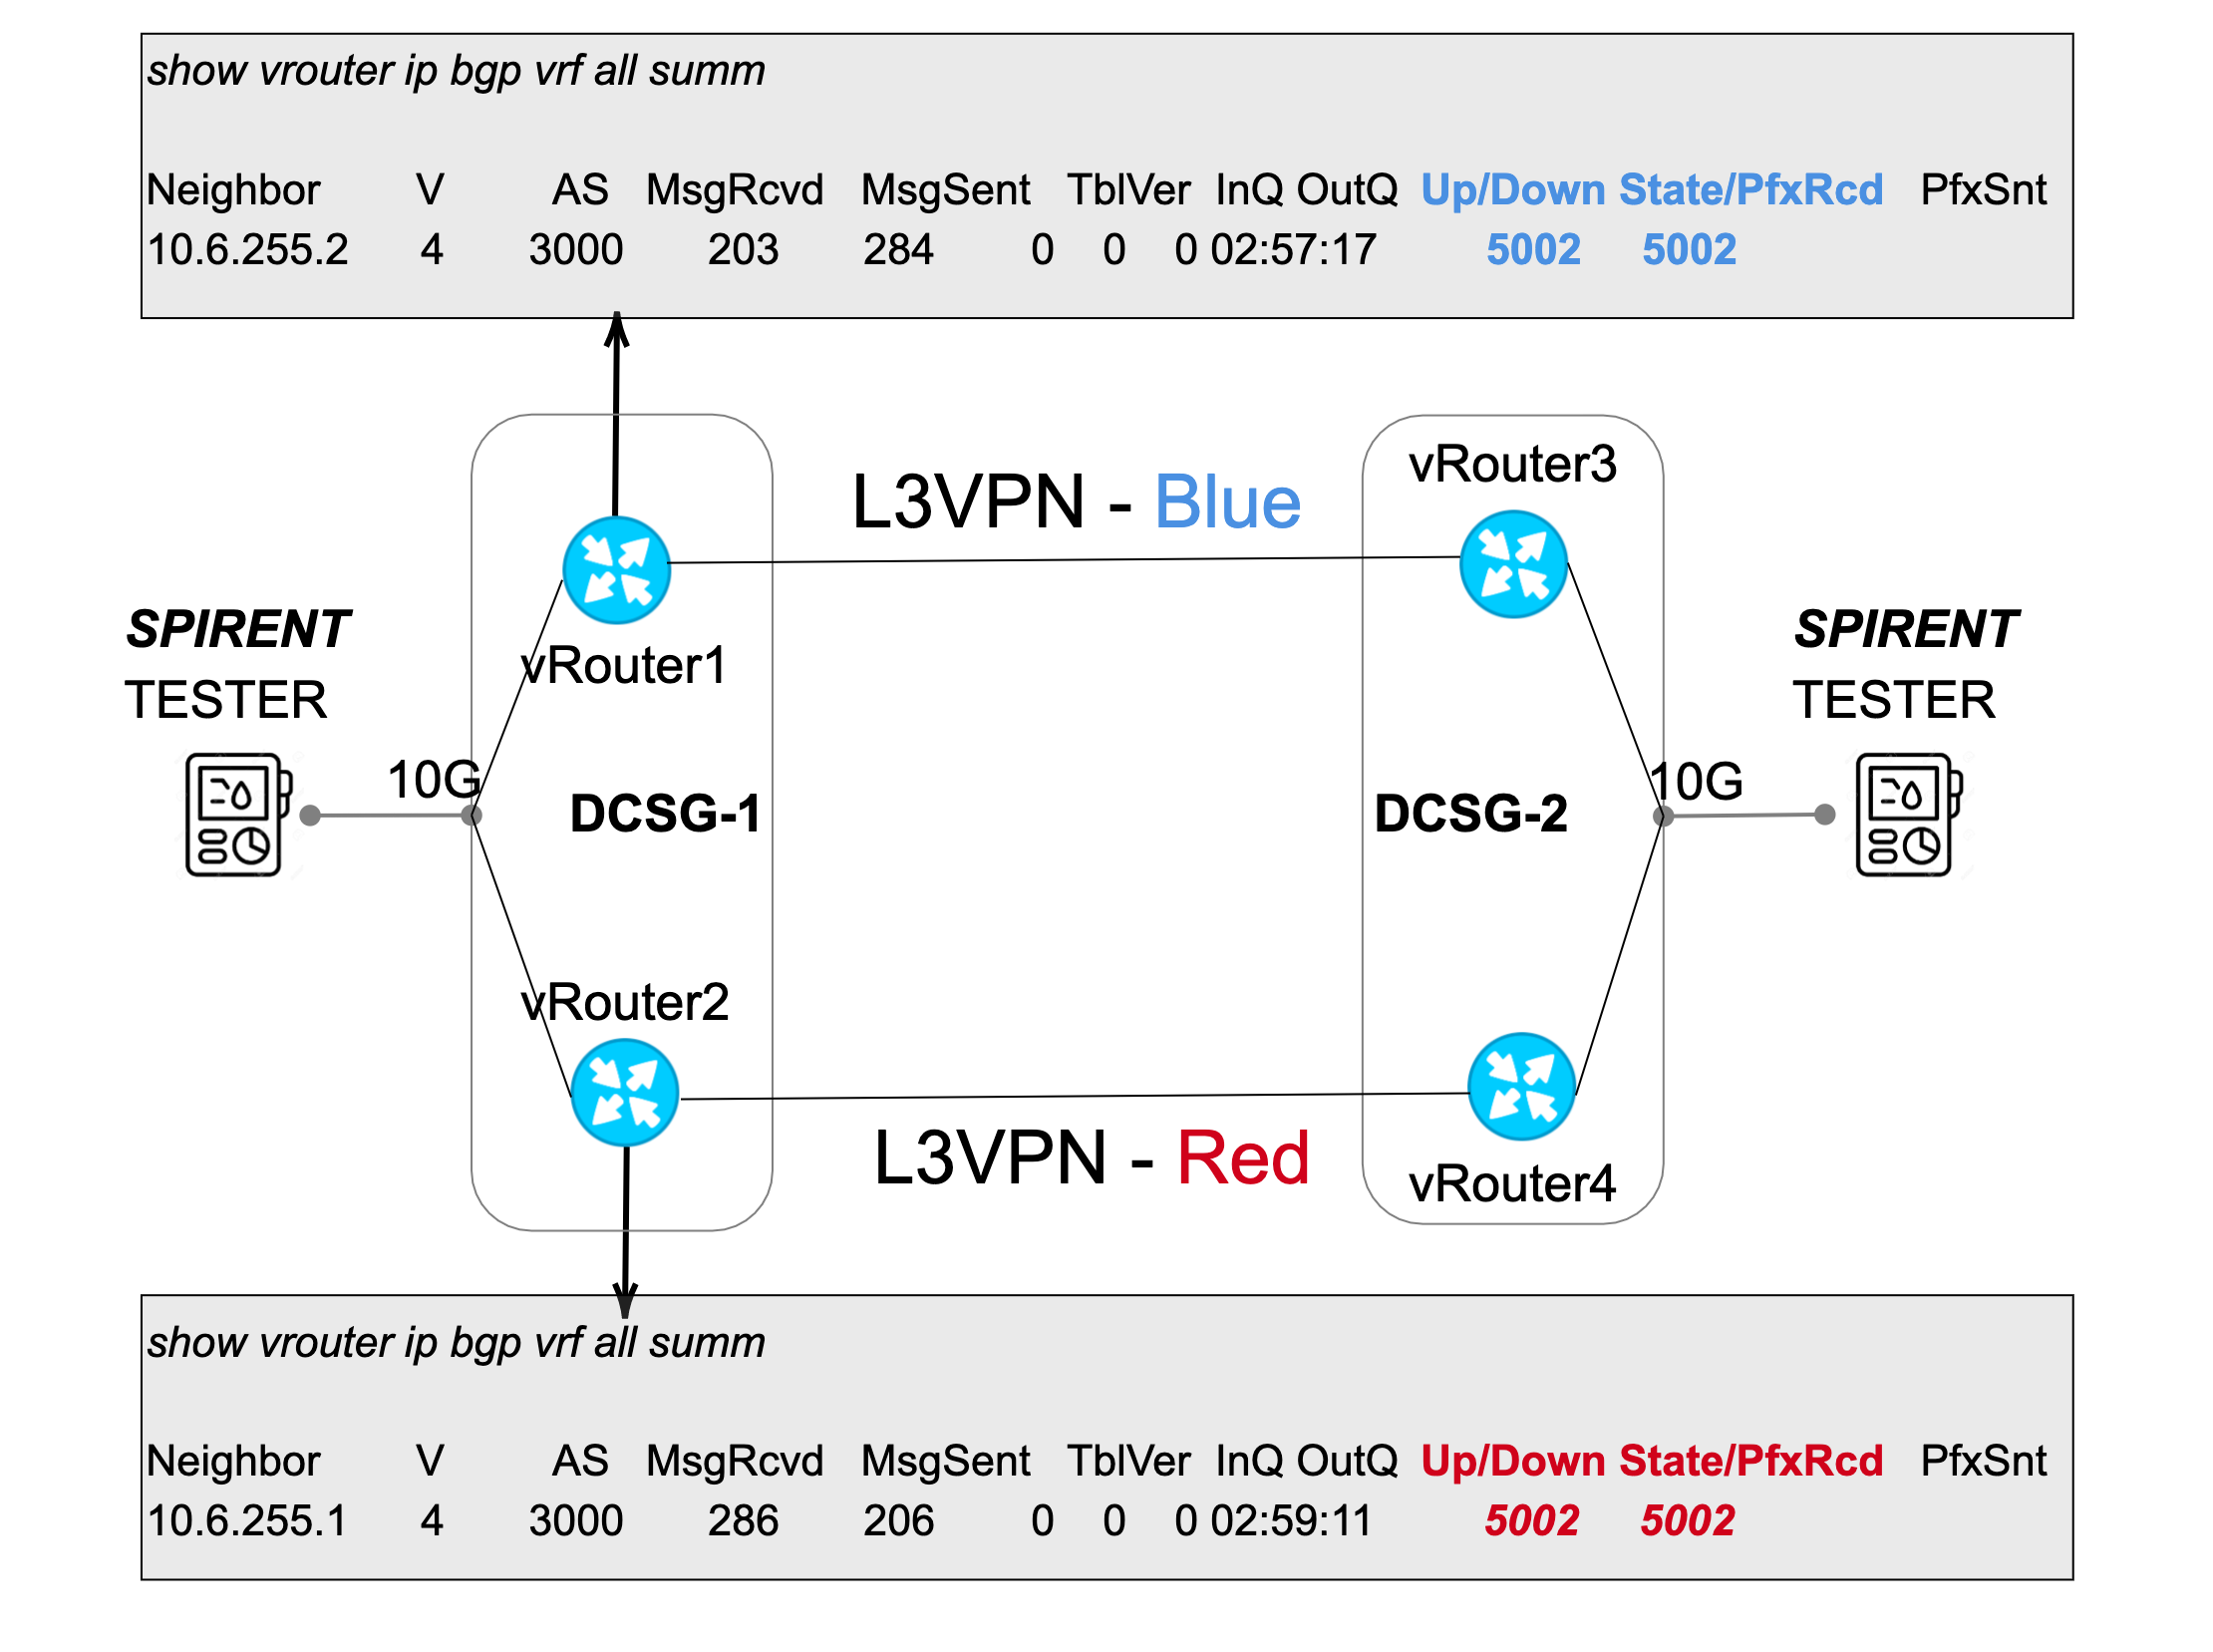
\includegraphics[width=\linewidth]{Figs/sliceresults.png}
\caption{Comparison of the Prefixes received and Sent in each of the network slices deployed in the network. Each Network slice (Blue and Red) has 5K prefixes announced.}
\label{fig:sliceresults}
\end{figure}

\begin{figure}[htb]
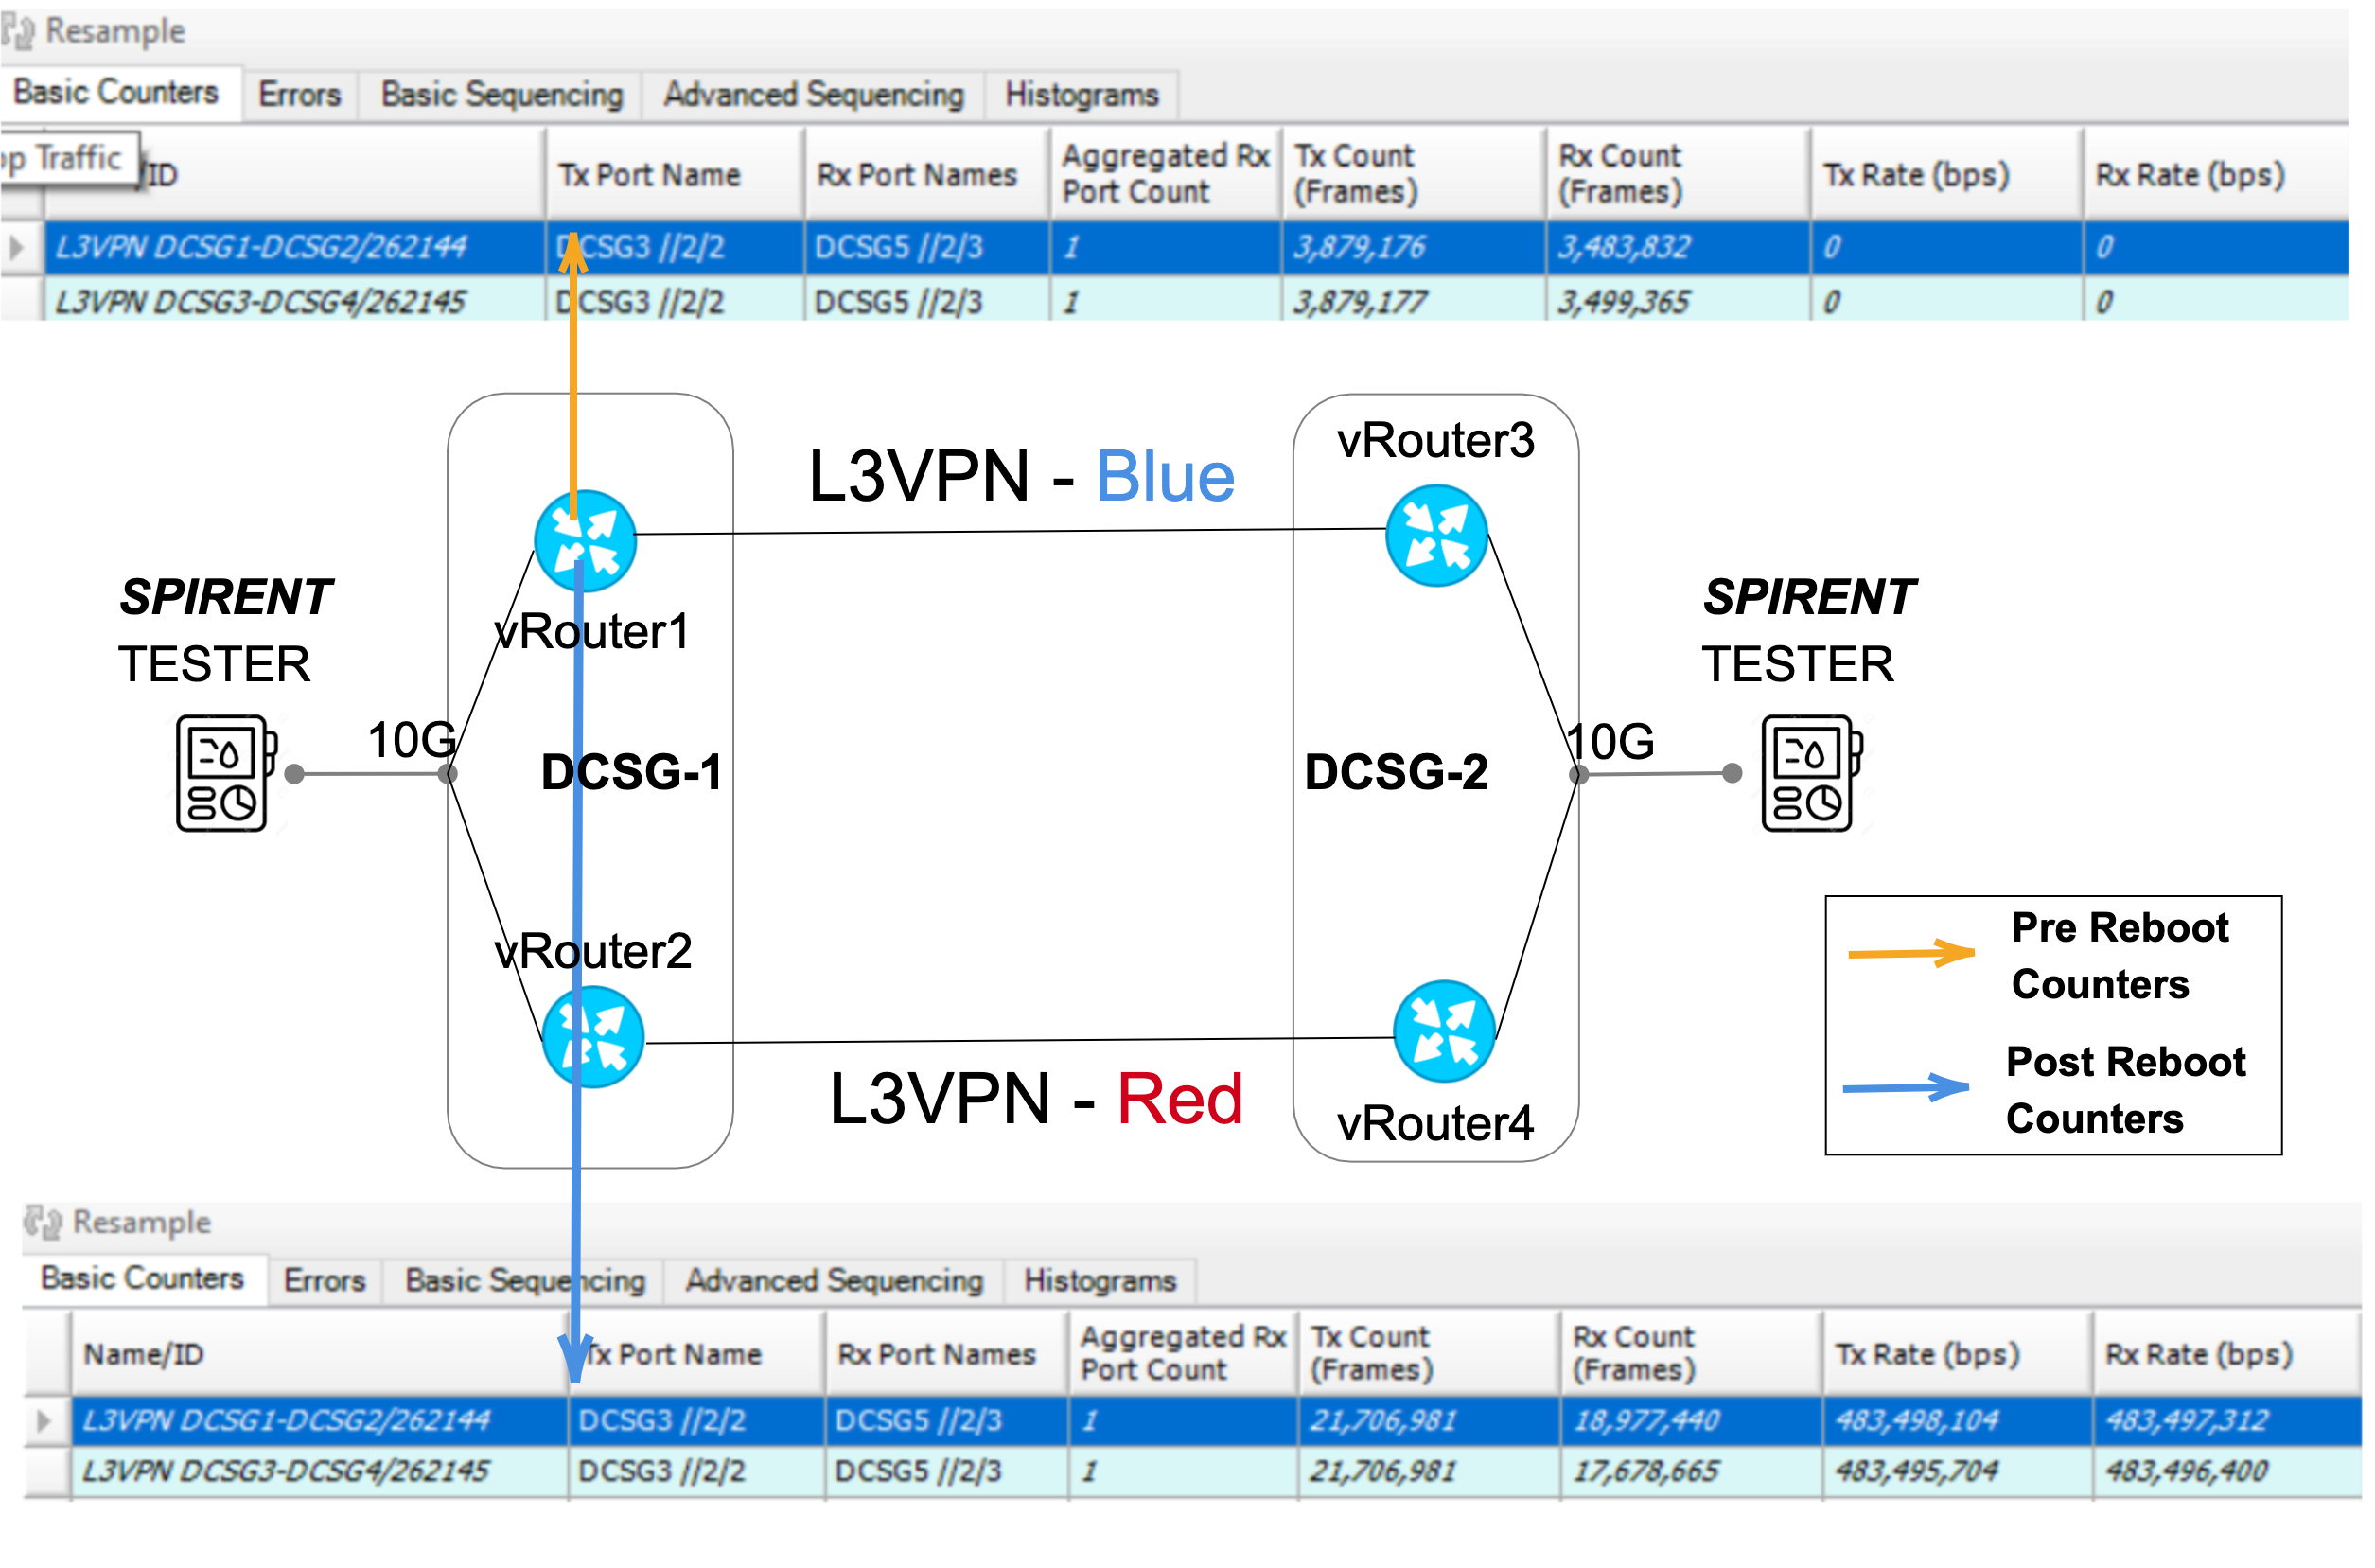
\includegraphics[width=\linewidth]{Figs/sliceresults2.png}
\caption{Depicts comparing the counters in the network slice Blue,  prior (Up) and after (Down) the device reboot. Once the devices are down, the counters go down to zero; after $4.6$ minutes and once the device is ready, the counters move up again. }
\label{fig:sliceresults2}
\end{figure}

After the end-to-end service creation and control and data plane validation, we have rebooted the devices to validate the service continuity after a simulated power failure. We validate that after the recovery was complete, all the traffic flows again between the network slices. To confirm the status of each device, we have captured the counters before and after the reboot process \cref{fig:sliceresults2}.  Each instance recovered sequentially, and it took up to $4.6$ minutes for the latest service to completely restore the traffic flow. 


%In order to properly set-up transport, we have introduced the transport network slice YANG data model in the RESTCONF server of NSC. An example of requested transport network slice is depicted in Figure \ref{fig:results}.c. It can be observed that several levels of isolation can be requested per node, link and slice. 
%In order to validate the depicted sequence diagram in Figure \ref{fig:scheme}.b, we provide the captured Wireshark traces among the complete system to deploy a complete hard slice request (the figure provides the selected significant traces). In this figure the different involved protocols can be observed. Firstly it shows the request for the transport network slice. It is quickly stored and answered, as it is processed after response (later an status update might be requested). 

%The transport network slice requests physical network isolation for the solicited link, thus a T-API connectivity service is requested including as connectivity constraints the diversity exclusion option. For that, we provide the identifiers from the previous established connectivity services and we obtain a disjoint path for the new requested slice, resulting in the requested physical network isolation (Figure \ref{fig:results}.b). It can be appreciated that the connectivity service setup time is 2.001s. Consider that the ADRENALINE testbed already has the paths equalized. 

%\begin{figure}[tb]%[htdp]
%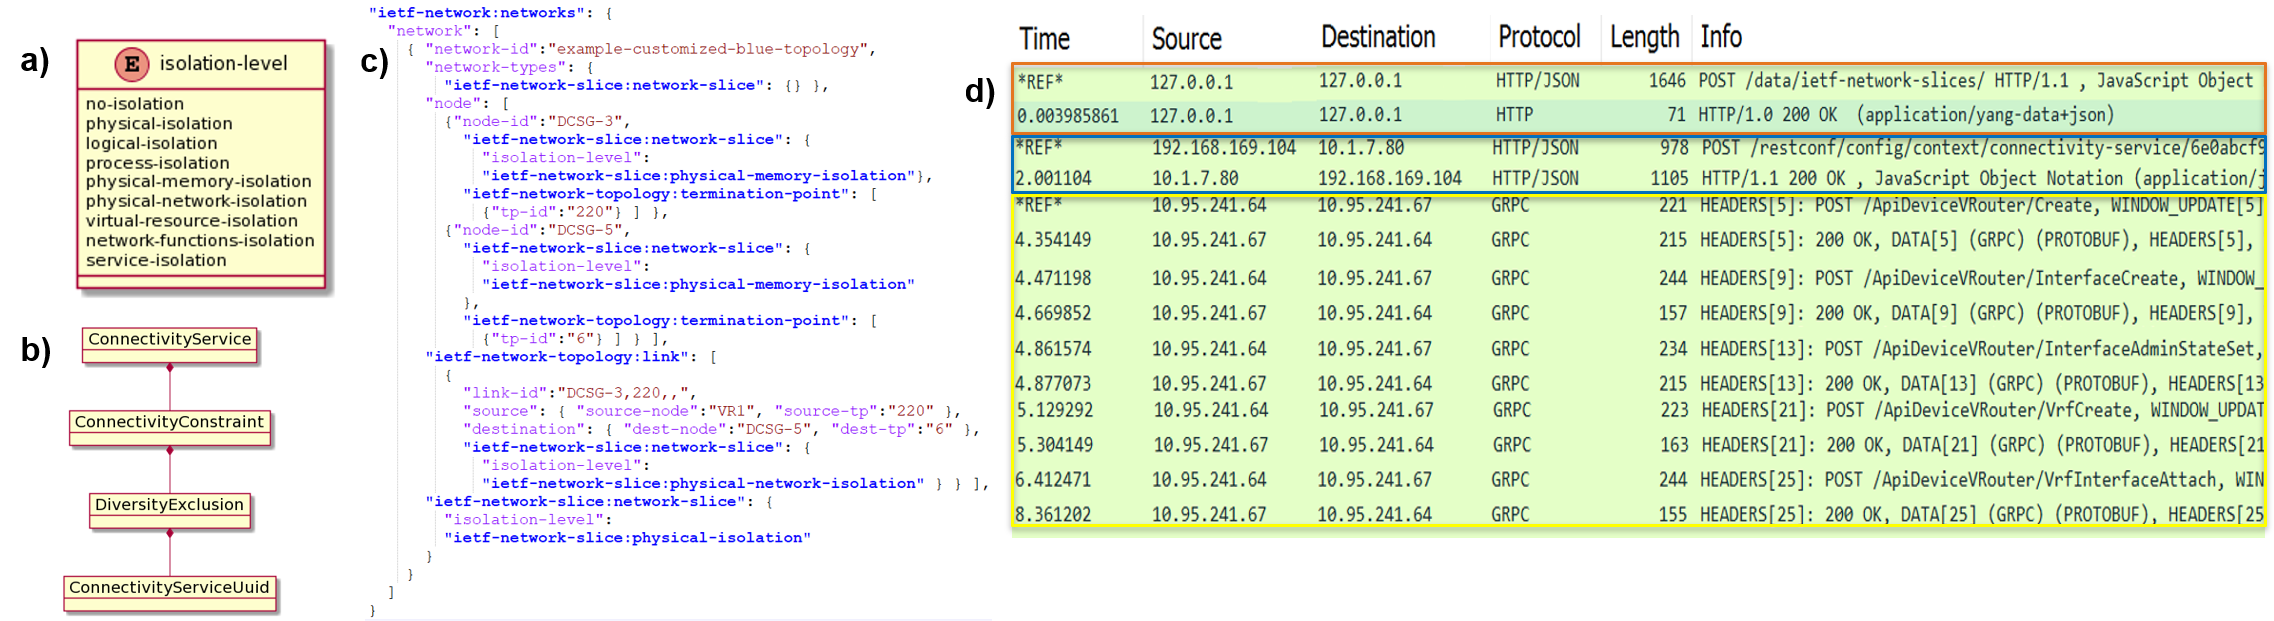
\includegraphics[width=\linewidth]{Figs/results.png}
%\caption{a) Network Slice isolation levels; b) Disjoint path selection using ONF Transport API; c) Example of transport slice request; and d) Wireshark captures for deployment of a hard slice.}
%\label{fig:results}
%\end{figure}

%Finally, the virtual routers (vRouter) are created and properly setup. The Wireshark capture shows the internal gRPC protocol from Volta Networks, which is equivalent to OpenConfig calls, for the vRouter deployment and configuration. It includes a call to create a new vRouter on top of Edgecore hardware. Then, interfaces are incorporated to the vRouter and configured. Later, Virtual routing and forwarding (VRF) table is setup and finally interfaces are attached to the VRF. This process set-up delay is of 8.36s. 



\section{Conclusions}
\label{sec:conclusions}

Dealing with the necessity of a dynamic network resources allocation to provide a new generation of customer-tailored applications is a primary concern nowadays. In that sense, Telecom providers have to prepare their whole set of systems and network infrastructure to allow the introduction of end-to-end network automation. In that sense, this paper uses and validates the iFusion architecture defined by Telefonica, which is ready to support new use cases derived from the 5G adoption and transport network slices. Additionally, this work validates an end-to-end creation, modification and deletion of transport network slices with several degrees of isolation. Furthermore, the results indicate the feasibility of deploying multi-layer IP over DWDM transport network slices based on virtual routers and disjoint optical paths.  Future work testing the map and realization of network slices in the different NSC controller positions is required. This testing would allow us to fully understand the information exchanged/stored in each layer to make feasible the deployments in real networks. 

%%%%%%%%%%%%%%%%%%%%%%%%%%%%%%%%%%%%%%%%%%

%\funding{Please add: ``This research received no external funding'' or ``This research was funded by NAME OF FUNDER grant number XXX.'' and  and ``The APC was funded by XXX''. Check carefully that the details given are accurate and use the standard spelling of funding agency names at \url{https://search.crossref.org/funding}, any errors may affect your future funding.}


\acknowledgments{Work partially supported by the EC H2020 TeraFlow (101015857) and Spanish AURORAS (RTI2018-099178-I00).}


\section{References}

% Please provide either the correct journal abbreviation (e.g. according to the “List of Title Word Abbreviations” http://www.issn.org/services/online-services/access-to-the-ltwa/) or the full name of the journal.
% Citations and References in Supplementary files are permitted provided that they also appear in the reference list here. 

%=====================================
% References, variant A: external bibliography
%=====================================
\externalbibliography{yes}
\bibliography{bibliography.bib}

%=====================================
% References, variant B: internal bibliography
%=====================================
%\begin{thebibliography}{999}
% Reference 1
%\end{thebibliography}

% If authors have biography, please use the format below
%\section*{Short Biography of Authors}
%\bio
%{\raisebox{-0.35cm}{\includegraphics[width=3.5cm,height=5.3cm,clip,keepaspectratio]{Definitions/author1.pdf}}}
%{\textbf{Firstname Lastname} Biography of first author}
%
%\bio
%{\raisebox{-0.35cm}{\includegraphics[width=3.5cm,height=5.3cm,clip,keepaspectratio]{Definitions/author2.jpg}}}
%{\textbf{Firstname Lastname} Biography of second author}

% The following MDPI journals use author-date citation: Arts, Econometrics, Economies, Genealogy, Humanities, IJFS, JRFM, Laws, Religions, Risks, Social Sciences. For those journals, please follow the formatting guidelines on http://www.mdpi.com/authors/references
% To cite two works by the same author: \citeauthor{ref-journal-1a} (\citeyear{ref-journal-1a}, \citeyear{ref-journal-1b}). This produces: Whittaker (1967, 1975)
% To cite two works by the same author with specific pages: \citeauthor{ref-journal-3a} (\citeyear{ref-journal-3a}, p. 328; \citeyear{ref-journal-3b}, p.475). This produces: Wong (1999, p. 328; 2000, p. 475)

%%%%%%%%%%%%%%%%%%%%%%%%%%%%%%%%%%%%%%%%%%
%% for journal Sci
%\reviewreports{\\
%Reviewer 1 comments and authors’ response\\
%Reviewer 2 comments and authors’ response\\
%Reviewer 3 comments and authors’ response
%}
%%%%%%%%%%%%%%%%%%%%%%%%%%%%%%%%%%%%%%%%%%
\end{document}

